
% This template was originally by R. Jacob Vogelstein
% Updated on March 1, 2010 by Noah J. Cowan


\documentclass[12pt,oneside,final]{thesis}

\newcommand{\pvec}[1]{\vec{#1}\mkern2mu\vphantom{#1}}

\usepackage{cite}
\usepackage[T1]{fontenc} %recommended to override the default font encoding package OT1
					%contains additional/standard ascii characters
\usepackage{amsmath, amsfonts, amssymb}
%it would be great if i could change the spacing above/below equations with a line here

\usepackage{braket}
\usepackage{siunitx}
\DeclareSIUnit{\torr}{Torr}
\DeclareSIUnit{\sccm}{sccm}
\DeclareSIUnit{\gram}{g}
\DeclareSIUnit{\rpm}{rpm}
\usepackage[version=3]{mhchem}
%\usepackage{textcomp}   %brought in for \textdegree on wiki recommendation
\usepackage{graphicx}
\graphicspath{{./figures/}}
\usepackage{fixltx2e}
\usepackage{array}
%\usepackage{wrapfig} 
%wrapfig is fragile: use sparingly
\usepackage[outdir=./figures/converted/]{epstopdf} 
%\usepackage{times}  % Use this for ugly fonts
\usepackage{fancyhdr}    % Use nice looking headers along with the required footer page numbers   
\usepackage{hyperref} %may require [hypertex] option

%Define the header/footer style
\pagestyle{fancy}
\fancyhf{}
\setlength{\headheight}{15pt}
\lhead{\leftmark}
\cfoot{\thepage}
\renewcommand{\headrulewidth}{0pt}
\fancypagestyle{plain}{% Redefine ``plain'' style for chapter boundaries
\fancyhf{} % clear all header and footer fields
\fancyfoot[C]{\thepage} % except the center
\renewcommand{\headrulewidth}{0pt}
\renewcommand{\footrulewidth}{0pt}}

%%This is a file for any additional functions that might need to be defined
%%It should be included in root.tex with %%This is a file for any additional functions that might need to be defined
%%It should be included in root.tex with %%This is a file for any additional functions that might need to be defined
%%It should be included in root.tex with \input{defs.tex}

%%Here is an example command that defines mass units

\newcommand{\gevcc}{\ifmmode \rm{GeV}/c^2%
                 \else%
                           \mbox{GeV}$/c^2$%
                 \fi%
                 }%

%%Here is an example command that defines mass units

\newcommand{\gevcc}{\ifmmode \rm{GeV}/c^2%
                 \else%
                           \mbox{GeV}$/c^2$%
                 \fi%
                 }%

%%Here is an example command that defines mass units

\newcommand{\gevcc}{\ifmmode \rm{GeV}/c^2%
                 \else%
                           \mbox{GeV}$/c^2$%
                 \fi%
                 }%

\tolerance=10000 %I don't know what this is for

%\makeglossary % enable the glossary

\begin{document}

\title{Fabrication and Transport Properties of Carbon Nanotube Quantum Dots with Ferromagnetic and Superconducting Leads}
\author{Nikolaus Hartman}
\degreemonth{August}
\degreeyear{2015} 
\dissertation
\doctorphilosophy
\copyrightnotice %not really copyrighted 


% add your chapters, best way is to have separate TeX files for each chapter
%% FRONTMATTER

\begin{frontmatter}

\maketitle

\begin{abstract}

Abstract here...

\vspace{1cm}

\noindent Primary Reader: Nina Markovic\\
Secondary Reader: N. Peter Armitage

\end{abstract}

\begin{acknowledgment}

Thanks \ldots

%Over the past seven years, whenever I have been asked why I chose to do my PhD work at Johns Hopkins I have had the same answer; the people here were by far the nicest and most helpful scientists I spoke with in making my decision. That has remained true throughout my career here. With that, the biggest thanks goes to my advisor, Nina Markovic. She was actually the first person I spoke with after accepting the offer here, only hours after accepting, just to let me know that there was room for another graduate student in her lab. She has consistently brought in big ideas for each of the graduate students in her lab. I could not have had an advisor with a personality I related to more than Nina. She was also always there to put me back in my place the moment I complained rather than getting back to work in the lab. That alone has gone a long way to making me a better scientist.
%
%During the time I spent in the Markovic lab I learned a great deal from my labmates. Soo Hyung Lee was here at the beginning to help me navigate the unfamiliar lab. Janice Guikema, throughout my time here, was always on hand to help me think about a problem or correct a sloppy technique. Similarly, our post doc Atikur Rahman provided huge amounts of measurement advice. I would not be able to cool down a single sample without what I learned from Atikur. Tyler Morgan-Wall has worked with me since nearly my first day in the lab. Rewiring cryostats, troubleshooting fabrication, and cooling a sample down until 2am would not have been half as much fun without him. JT Mlack came in a two years later, and was always on hand to discuss sci-fi, samples, and remind me I might take things a little too seriously. 
%
%In addition to my labmates, there are too many other physicists and Baltimoreans to thank. Thanks to Dan Allan, Dan Richmond, and Nuala McCullagh for suffering through the first year and more with me. Seamus Riley, Jess Brick, Laura McDonald, Sarah LaRocca, Andrew Whitbeck, and Stefan Byrd-Kreuger, our time at the Meat Castle, Countdown, and New Years cabins was phenomenal. Thanks to every other physicist in Bloomberg who has helped maintain the social, collaborative atmosphere that brought me here.
%
%Thanks to my family, my parents Ann and George, and my sister Erika, who were unfailingly supportive of my work on toward this PhD. Finally, thanks to Stephanie, who has put up with watching me struggle to finish the PhD for quite some time without ever losing her signature cheerful outlook.

\end{acknowledgment}

%\begin{dedication}
% 
%This thesis is dedicated to \ldots
%
%\end{dedication}

% generate table of contents
\tableofcontents

% generate list of tables
\listoftables

% generate list of figures
\listoffigures

\end{frontmatter}
  % title, abstract, acknowledgement, dedication, TOC, figure list
\chapter{Introduction}
\label{sec:intro}
\chaptermark{Introduction}

This thesis work focuses on a narrow range of fabrication techniques and electronic transport measurements on a specific type of mesoscopic device, carbon nanotube quantum dots. In this introduction, the motivations behind this work will be explained along with an outline of what is to be discussed. 

\section{Transport Spectroscopy in Quantum Dots}

Using transport spectroscopy to probe low energy density of states can yield a great deal of insight into the nature of the materials being probed. A simple conductance measurement through two materials and a tunnel barrier measures a convolution of the density of states for each of the materials, $N_1(E)$ and $N_2(E)$.

\begin{equation}
    \label{eq:conductance}
    G \sim \int N_1(E) N_2(E)\frac{df(E+eV)}{dV}dE
\end{equation}

At low temperatures, the derivative of the Fermi function is approximated by a delta function and provides a sharp kernel for this convolution. By measuring the conductance across the junction, much can be learned about the nature of the materials, such as in the work of Tedrow and Meservey on measuring the polarization of magnetic materials \cite{Tedrow1971}

By using making a two junction device, and introducing a constriction in the intermediate material, either through local gating or by using low dimensional materials, an interesting situation is created. At low temperatures, the confinement of electrons in the constriction will dominate the transport. Consider an electron confined within a one dimensional length, $L$. The electron has energies on the order of $E \sim \hbar^2k \pi^2/2mL^2$. For length scales smaller than 100nm and $k_B T < E$ ,the quantum mechanical levels in the constriction dominate the electron transport through the device. The measured conductance will show discrete levels corresponding to the filling of the quantum levels in the constriction. This device is called a quantum dot.

Calculating the electron transport properties through a quantum dot is considerably more complicated than the application of Equation \ref{eq:conductance}. At small sizes and low temperatures, not only is the filling of the quantum levels in the dot important, but the electron-electron interactions on the dot must be considered, as well as the interactions between the dot, the two materials connected to it through tunnel barriers, and any electrostatic gates. The Hamiltonian for such a quantum dot with $N$ electrons looks like \cite{Ihn2004}:

\begin{equation}
\label{eq:full_hamiltonian}
    H_N = \sum_{n=1}^N \left( \frac{\mathbf{p}_n^2}{2m^*} - e \int_V dV \rho_{ion}(\mathbf{r})G(\mathbf{r}_n, \mathbf{r}) + \frac{e^2}{2} G(\mathbf{r}_n, \mathbf{r}) - e \sum_i \phi_i \alpha_i (\mathbf{r}_n) + e^2 \sum_{m=1}^{n-1} G(\mathbf{r}_m, \mathbf{r}_n) \right)
\end{equation}

In order, these terms describe the kinetic energy of the electrons, the energy of interactions with fixed ions in the system, image charge potential for an individual electron, changes in potential energy from interaction with $i$ gate electrodes, and a self-energy term that should be renormalized away. Obviously, comparing every experiment to this model is impractical and unnecessary. Section \ref{sec:constant_interaction_model} will introduce the simplest model for capturing quantum dot behavior, called the constant interaction model. In that, the Hamiltonian above is simplified such conductance through the dot only depends on the energy levels on the dot, as calculated with basic quantum mechanics, and the total capacitance of the device, which takes the place of all the electrostatic terms in Equation \ref{eq:full_hamiltonian}. Chapter \ref{sec:CNT} will discuss the basic behavior, at room temperature and low temperatures, of carbon nanotube quantum dot devices in terms of the constant interaction model.

The constant interaction model can be expanded by adding asymmetric, spin dependent tunnel barriers, and spin interactions between electrons in different energy levels confined to the same dot. This is the case when quantum dots are formed using ferromagnetic and superconducting materials. The interplay between magnetism, superconductivity, and transport through a quantum dot is the focus of much of this thesis. 

\section{Working with Carbon Nanotubes}

Carbon nanotube quantum dots are an ideal platform for making the type of transport measurements described above. They are inherently one dimensional conductors with diameters on the order of 1nm. The large aspect ratio of carbon nanotubes (>1000:1) leaves plenty of room to fabricate the metallic contacts needed for transport measurements along the nanotube length.

Building carbon nanotube quantum dot devices tends to be a very personal experience. Each young scientist has a list of recipes, opinions, and techniques with a wide range of scientific and quasi-religious motivations. Occasionally, this effort results in gorgeous datasets and rich physics. Once this happens, the hundreds of devices built, and subtle techniques tested, leading to the publication are quickly forgotten in favor of the results. The lack of transparency hinders reproducibility and progress in the field. An effort has been made in this thesis to explain, in detail, all of the techniques used in fabrication and comment on their reproducibility.

\section{Current Work}

Chapters \ref{sec:growth} and \ref{chap:contacts} document a variety of nanotube growth and contact fabrication techniques tested in this work. Chapter \ref{sec:growth} discusses  efforts made in our lab to replicate a number of nanotube growth recipes. In Chapter \ref{chap:contacts}, statistics on the devices made, their fabrication steps, and resulting measurements are discussed. The large volume of devices fabricated allows for a meaningful comparison of fabrication techniques that has not previously been seen. Improved imaging and sample processing techniques are also developed in this chapter. Additionally, a discussion of noise sources in the resulting devices is presented. Recommendations for fabrication are made based on the data analysis.

Chapters \label{sec:FMCNTQD} and \label{sec:SCFM} discuss spin-dependent, low-temperature, transport measurements on carbon nanotube quantum dot devices with ferromagnetic and superconducting contacts. In ferromagnetic devices, we were able to test a number models proposed in previous work and observe the appearance of conductance suppression and negative differential conductance based on spin selection rules. The F-CNT-S show evidence of proximity induced superconductivity as well as magnetic field dependent fluctuations in transport through the quantum dot. These measurements are the first attempt to analyze conductance through such a device.

  % an introduction to the field and some bullshit to tie the whole thing together
%% This is going to be my carbon nanotube chapter. It should be based almost completely on GBO notes

\chapter{Electronic Properties of Carbon Nanotubes}
\label{sec:CNT}
\chaptermark{Properties of CNTs}

Carbon nanotubes exhibit a variety of interesting material and electrical properties. Nanotubes can be used as mechanical oscillators, one dimensional conductors, and quantum dots, among many other applications. The work in this thesis takes advantage of the unique electronic and spin transport properties of carbon nanotubes. By starting with the graphene lattice, these properties are easily derived. 

\section{Electronic Bandstructure of Graphene}

The electronic bandstructure of graphene was first calculated in 1947 by P.R. Wallace (CITE). This was done as part of an effort to understand the electronic structure of bulk graphite. In this paper, there is mention of the two lowest energy bands and the half filling of a single layer of carbon atoms. It was not until 1984 that Semenoff discussed the existence of a linear dispersion relation for low energy electronic excitations in single layers of carbon atoms (CITE). This was done by looking at a generic honeycomb lattice as an analoge of 2+1 dimensional electrodynamics. Semenoff found the low energy electronic band structure of the monoatomic honeycomb lattice matched that of Dirac fermions.

Graphene was first isolated on silicon wafers through mechanical exfoliation in 2004. The semimetallic characteristics were confirmed through measuring transistor curves and the charge carrier sign change through the Hall effect (CITE). Shortly after, the same research group confirmed the existance of low energy Dirac fermions in graphene (CITE).

Beginning with the structure of the monoatomic honeycomb lattice, and following the original work of Wallace, the electronic band structure of graphene will be derived below.

\subsection{Graphene Lattice}

As mentioned above, single layers of carbon atoms, graphene, form a honeycomb lattice. This lattice can be seen in Figure \ref{fig:graphene_unit_cell}.

\begin{figure}
    \centering
    \includegraphics[width = 0.5\textwidth]{chapter2/graphene_unit_cell.png}
    \caption{The real-space structure of the graphene lattice. Vectors $\vec{a}_1$ and $\vec{a}_2$ define the unit cell, which contains two atoms, highlighted in red and blue.}
    \label{fig:graphene_unit_cell}
\end{figure}

In Figure \ref{fig:graphene_unit_cell} the unit cell is defined by the two lattice vectors $\vec{a}_1$ and $\vec{a}_2$. Each unit cell is comprised of two atoms. The honeycomb lattice can be thought of as to interpenetrating triangular sublattices. With that picture, the honeycomb unit cell contains one atom from each of the two sublattices, highlighted in Figure \ref{fig:graphene_unit_cell} as red (A) and blue (B). Each atom on the lattice contributes one conduction electron.

Using the coordinates defined in Figure \ref{fig:graphene_unit_cell}, the lattice vectors are defined, from the center of a honeycomb.

\begin{align}
    \vec{a}_1 &= \frac{3a_0}{2}\hat{i} + \frac{\sqrt{3}a_0}{2}\hat{j} \\
    \vec{a}_2 &= \frac{3a_0}{2}\hat{i} - \frac{\sqrt{3}a_0}{2}\hat{j}
\end{align}

Here $a_0$ is the carbon-carbon bond distance, \SI{1.42}{\angstrom} (CITE).

The reciprocal lattice vectors, $\vec{b}_1$ and $\vec{b}_2$ can now be found in the usual way.

\begin{equation}
    a_i \cdot b_j = 2\pi \delta_{ij}
\end{equation}

Here $\delta_{ij}$ is the Kronecker delta. The reciprocal lattice defined by $\vec{b}_1$ and $\vec{b}_2$ can be seen in Figure \ref{fig:graphene_k_space}.

\begin{align}
    \vec{b}_1 &= \frac{2\pi}{3a_0}\hat{i} + \frac{2\sqrt{3}\pi}{3a_0}\hat{j} \\
    \vec{b}_2 &= \frac{2\pi}{3a_0}\hat{i} - \frac{2\sqrt{3}\pi}{3a_0}\hat{j}
\end{align}

\begin{figure}
    \centering
    \includegraphics[width = 0.5\textwidth]{chapter2/graphene_k_space.png}
    \caption{The reciprocal lattice of graphene. Vectors $\vec{b}_1$ and $\vec{b}_2$ define the Brillouin zone. The high symmetry points $\Gamma$, $K$, $K'$, and $M$ are labeled.}
    \label{fig:graphene_k_space}
\end{figure}

The reciprocal lattice is also a honeycomb lattice, rotated 90 degrees from the real space lattice. The size of each Brillouin zone is defined by the reciprocal lattice vectors above. A few high symmetry points have been labelled in the figure. Of particular note are the three $K$ and three $K'$ points. As will be seen in the band structure calculation, these are the points at which the conduction and valence bands will meet to form the Dirac cones that give rise to graphene's interesting low energy conduction properties.

\subsection{Tight Binding Model}

The simplest way to calculate the low energy electronic band structure for graphene is using a nearest neighbor tight binding model, also known as a linear combination of atomic orbitals (CITE). In this model, each conduction electron is tightly bound to a lattice site with a small probability of hopping only to a nearest neighbor site. With this simple picture for electron conduction, one can find the lowest energy bands in graphene.

Given that the model deals with the motion of individual electrons and their wavefunctions at each atomic site, the goal will be to solve the time independent Schr\"{o}dinger equation.

\begin{equation}
    \hat{H}\Psi = \varepsilon\Psi
\end{equation}

$\Psi$ is a single particle wavefunction over the whole graphene lattice. As such, it can be written as a linear combination of Bloch wavefucntions.

\begin{align}
    u_A(\vec{r}) &= \frac{1}{\sqrt{N}}\sum_{\vec{r}_A}^{} e^{i\vec{k}\cdot\vec{r}_A} \phi_{2p_z}(\vec{r}-\vec{r}_A) \\
    u_B(\vec{r}) &= \frac{1}{\sqrt{N}}\sum_{\vec{r}_B}^{} e^{i\vec{k}\cdot\vec{r}_B} \phi_{2p_z}(\vec{r}-\vec{r}_B)
\end{align}

These two functions represent Bloch waves localized on the A and B sublattices, respectively. With these definitions the full single-particle wavefunction can be rewritten as follows:

\begin{equation}
    \Psi = C_A u_A + C_B u_B
\end{equation}

$C_{A(B)}$ represents the amplitude of the wavefunction on the A(B) sublattice. With all of the above definitions the time independent Schr\"{o}dinger equation can be rewritten in a matrix form:

\begin{equation} 
\label{eq:TISE}
    \begin{pmatrix} H_{AA} & H_{AB} \\ H_{BA} & H_{BB} \end{pmatrix} \begin{pmatrix} C_A \\ C_B \end{pmatrix} = \varepsilon \begin{pmatrix} S_{AA} & S_{AB} \\ S_{BA} & S_{BB} \end{pmatrix} \begin{pmatrix} C_A \\ C_B \end{pmatrix}
\end{equation}

Where:

\begin{align}
\label{eq:matel}
    H_{ij} &= \braket{u_i | H | u_j} \\
    S_{ij} &= \braket{u_i | u_j}
\end{align}

For simplicity, the rest of this calculation will assume $\braket{u_i | u_j} = \delta_{ij}$. Meaning, there is no overlap of the two Bloch wavefunctions and that each of the wave functions is already properly normalized. Rewriting Equation \ref{eq:TISE} yields:

\begin{equation}
\label{eq:secular}
    \begin{pmatrix} H_{AA}-\varepsilon & H_{AB} \\ H_{BA} & H_{BB}-\varepsilon \end{pmatrix} \begin{pmatrix} C_A \\ C_B \end{pmatrix} = 0
\end{equation}

Non-trival solutions to Equation \ref{eq:secular} exist only when:

\begin{equation}
\label{eq:eigenvals}
    \begin{vmatrix} H_{AA}-\varepsilon & H_{AB} \\ H_{BA} & H_{BB}-\varepsilon \end{vmatrix} = 0
\end{equation}

Solving equation \ref{eq:eigenvals} gives the energy eigenvalues in terms of the matrix elements defined in equation \ref{eq:matel}.

\begin{equation}
\label{eq:simple_bands}
    \varepsilon = H_{AA} \pm \lvert H_{AB} \rvert
\end{equation}

Where the relations $H_{AA} = H_{BB}$ and $H_{AB} = {H^*}_{BA}$ were used.

In order to obtain a useful expression for the energy bands in terms of the electron momentum $\vec{k}$, Equation \ref{eq:simple_bands} must be simplified using the expressions for the Bloch wavefunctions. 

\begin{align}
    H_{AA} &= \frac{1}{N} \sum_{\vec{r}_A}^{} \sum_{\pvec{r}'_A}^{} e^{i \vec{k}\cdot(\vec{r}_A - \pvec{r}'_A)} \int \phi^*_{2p_z}(\vec{r}-\vec{r}_A) \hat{H} \phi_{2p_z}(\vec{r}-\pvec{r}'_A) \, d^3\vec{r} \label{eq:overlap_AA} \\
    H_{AB} &= \frac{1}{N} \sum_{\vec{r}_A}^{} \sum_{\vec{r}_B}^{} e^{i \vec{k}\cdot(\vec{r}_A - \vec{r}_B)} \int \phi^*_{2p_z}(\vec{r}-\vec{r}_A) \hat{H} \phi_{2p_z}(\vec{r}-\vec{r}_B) \, d^3\vec{r} \label{eq:overlap_AB}
\end{align}

The summation in Equation \ref{eq:overlap_AA} can be evaluated to yield:

\begin{equation}
\label{eq:pz_energy}
    H_{AA} = \int \phi^*_{2p_z}(\vec{r}-\vec{r}_A) \hat{H} \phi_{2p_z}(\vec{r}-\vec{r}_A) \, d^3\vec{r} = \varepsilon_{p_z}
\end{equation}

Where $\varepsilon_{p_z}$ is the energy of a single electron on a $p_z$ orbital. For the sake of simplicity, the rest of this chapter will assume $\varepsilon_{p_z} = 0$. 

In order to simplify Equation \ref{eq:overlap_AB} it is useful to define the vectors pointing from an atom on the B sublattice to its three nearest neighbors on the A sublattice.

\begin{align}
    \vec{\delta}_1 &= \frac{1}{3}(2\vec{a}_1 - \vec{a}_2) = \frac{a_0}{2}\hat{i} + \frac{\sqrt{3}}{2}a_0\hat{j} \nonumber \\
    \vec{\delta}_2 &= \frac{1}{3}(2\vec{a}_2 - \vec{a}_1) = \frac{a_0}{2}\hat{i} - \frac{\sqrt{3}}{2}a_0\hat{j} \label{eq:deltas} \\
    \vec{\delta}_3 &= -\frac{1}{3}(\vec{a}_1 + \vec{a}_2) = -a_0\hat{i} \nonumber
\end{align}

With these definitions Equation \ref{eq:overlap_AB} can be rewritten as:

\begin{equation}
\label{eq:AB_simple}
    \hat{H}_{AB} = \sum_{i=1}^{3} e^{i\vec{k}\cdot\vec{\delta}_i} \int \phi^*_{2p_z}(\vec{r}) \hat{H} \phi_{2p_z}(\vec{r}-\vec{\delta}_i) \, d^3\vec{r}
\end{equation}

Since the exact form of the Hamiltonian is not known, the integral in Equation \ref{ep:AB_simple} cannot be evaluated. However, the integral clearly represents the overlap between the wavefunction of an electron in a $p_z$ orbital on the A lattice and its nearest neighbor on the B lattice. With that in mind, the hopping amplitude $t$ is defined:

\begin{equation}
\label{eq:hopping_amp}
    t = \int \phi^*_{2p_z}(\vec{r}) \hat{H} \phi_{2p_z}(\vec{r}-\vec{\delta}_i) \, d^3\vec{r}
\end{equation}

Note, there is only one hopping amplitude, independent of the index $i$, since the distance between all nearest neighbors, $\lvert \delta_i \rvert$, is the same. With this definition, the overlap integral can be rewritten once more.

\begin{equation}
\label{eq:AB_final}
    H_{AB} = t \sum_{i=1}^{3} e^{i\vec{k}\cdot\vec{\delta}_i}
\end{equation}

Equation \ref{eq:AB_final} can be combined with the assumption that the onsite energy can be set to zero, $\varepsilon_{p_z} = 0$ to give the final effective Hamiltonian for this model.

\begin{equation}
\label{eq:effective_H}
    \hat{H} = \begin{pmatrix} 0 & t \sum_{i}^{} e^{i\vec{k}\cdot\vec{\delta}_i} \\  t \sum_{i}^{} e^{-i\vec{k}\cdot\vec{\delta}_i} & 0 \end{pmatrix}
\end{equation}

Using these same results in Equation \ref{eq:simple_bands} gives the two lowest energy bands in terms of the hopping amplitude, $t$. 

\begin{equation}
    \varepsilon(\vec{k}) = \pm t \left| \sum_{i}^{} e^{i \vec{k}\cdot\vec{\delta}_i} \right| \nonumber \\
\end{equation}
\begin{equation}
    \varepsilon(\vec{k}) = \pm t \sqrt{ 1 + 4\cos\left(\frac{3a_0}{2}k_x\right)\cos\left(\frac{\sqrt{3}a_0}{2}k_y\right) + 4\cos^{2}\left(\frac{\sqrt{3}a_0}{2}k_y\right)} \label{eq:bands}
\end{equation}    

These two bands can be seen in Figure \ref{fig:graphene_bands}. 

\begin{figure}
    \centering
    \includegraphics[width = 1.0\textwidth]{chapter2/graphene_band_fig.png}
    \caption{(a) The $\pi$-bands of graphene calculated using a nearest neighbor tight binding model. (b) A contour plot of the lower band with the first Brillouin zone drawn. The bands meet at the three $K$ and three $K'$ points at the vertices of the Brillouin zone.}
    \label{fig:graphene_bands}
\end{figure}

\subsection{Low Energy Bandstructure of Graphene}



\section{Carbon Nanotube Quantum Dots}

How to interpret/understand quantum dot measurements. % derivation of CNT band structure, explanation of QD + measurements
%% all about growing, placing, imaging, filtering carbon nanotubes

\chapter{Carbon Nanotube Growth and Placement}
\label{sec:growth}
\chaptermark{Growth and Placement}

In the years since their discovery, many methods of producing electronic devices from carbon nanotubes have been developed. These include random dispersion (Section \ref{sec:random_dispersion}), on-substrate catalyst island growth (Section \label{sec:catalyst_island}) and stamping \cite{Wu2010, Pei2012}. For this work, the first two methods were successfully used to produce carbon nanotube quantum dots. It was found that the catalyst island growth was much easier to implement and required much less processing time per device.

\section{Random Dispersion}
\label{sec:random_dispersion}

The first successful method of nanotube device fabrication was what will be referred to here as random dispersion. First, nanotubes are grown in bulk through chemical vapor deposition (or other preferred method). Then, the nanotubes are suspended in a solution. Finally, the nanotubes are cast onto a substrate. Nanotubes can then be located relative to some predefined markers on the substrate.

\subsection{Catalyst}
\label{subsec:disperse_catalyst}

All of the devices discussed in this thesis have utilized the same, iron-based catalyst \cite{Kong1998, Kong1998a}. The simplest way to create this catalyst is to combine the ingredients in Table \ref{table:powder_catalyst} in a mortar and pestle and grind until it turns a uniform dark orange color. Adding some additional alumina seems to promote growth of longer tubes, possibly by lowering the density of tubes grown from each alumina/iron/molybdenum particle.

\begin{table}
	\centering
	\caption{Powder Catalyst}
    \begin{tabular}{ c | c }
    	\hline
        \ce{Fe(NO3)3*9H2O} & \SI{20}{\milli\gram} \\ \hline
        \ce{MoO2(acac)2} & \SI{5}{\milli\gram} \\ \hline
        \ce{Al2O3} & \SI{15}{\milli\gram} \\ \hline
    \end{tabular}
    \label{table:powder_catalyst}
\end{table}

\subsection{Growth}
\label{subsubsec:powder_cvd}

Of the many possible techniques for nanotube growth, we choose chemical vapor deposition for its simple implementation. The process is carried out in a Lindberg Blue tube furnace using a 1 inch diameter quartz tube. The furnace, quartz tube, and exhaust filtering are seen in Figure~\ref{fig:furnace_setup}. This setup has been repeatedly, and successfully, leak checked. Oxygen leaks can be detrimental to the nanotube growth process by forming \ce{CO} and \ce{CO2} with any free carbon, and potentially causing a fiery reaction with free hydrogen from the methane decomposition.

\begin{figure}
    \centering
    \includegraphics[width = 0.8\textwidth]{chapter3/furnace_setup.jpg}
    \caption{The tube furnace fitted with a 1" diameter quartz tube. The tube is sealed at both ends using 1" rubber tubing, cable clamps, and KF25 fittings. Gas flows from left to right in the picture. The gas flows out of the furnace into a mineral oil bubbler to keep hot hydrogen from reaching the air in the room. Gas then flows from the bubbler into the building exhaust.}
    \label{fig:furnace_setup}
\end{figure}

The gases used in the CVD process, argon, hydrogen, and methane, are fed into the furnace using a custom-made gas handling panel. The panel has three gas channels, each with its own analog flowmeter, needle valve, and on/off valve. A digital flowmeter placed at the right side of the panel reads the total flow of combined gas exiting the panel to the furnace. The gas handling panel can be see in Figure~\ref{fig:gas_panel}

\begin{figure}
    \centering
    \includegraphics[width = 0.8\textwidth]{chapter3/gas_panel.jpg}
    \caption{The gas handling panel for our Lindberg tube furnace. Gas flow is from left to right.}
    \label{fig:gas_panel}
\end{figure}

The growth procedure begins with filling a ceramic crucible with the iron catalyst described in \ref{subsec:disperse_catalyst}. The catalyst should be spread in a thin layer across the bottom of the crucible, which is then loaded into the center of a 2-4 foot long quartz tube. The tube is sealed at each end, one side connected to the gas handling panel, and the other connected to the mineral oil filter and building exhaust. Our standard nanotube growth recipe is as follows: 

%can i remove the spacing from between these list items?
\begin{enumerate}
	\item Purge the tube by flowing \SI{2000}{\sccm} of Ar for 20 minutes
	\item Heat tube to \SI{1000}{\degreeCelsius} while flowing \SI{1000}{\sccm} Ar and \SI{200}{\sccm} \ce{H2}
	\item Flow \SI{2000}{\sccm} \ce{CH4} and \SI{200}{\sccm} \ce{H2} for 10 minutes.
	\item Set temperature to \SI{0}{\degreeCelsius} and let the furnace cool while flowing \SI{1000}{\sccm} Ar and \SI{200}{\sccm} \ce{H2}
\end{enumerate}

\noindent The actual nanotube growth occurs during the methane flow step. The \SI{200}{\sccm} \ce{H2} flow can be omitted, but it does seem to help promote nanotube growth. The flow rates do not need to be precise. Most nanotubes grow in the first few seconds of methane flow regardless of the flow rate. The Ar and \ce{H2} are simply to keep \ce{O2} and \ce{H2O} out of the tube. 

\subsection{Nanotube Placement}

After the CVD process, the nanotubes remain attached to the iron\slash alumina\slash molybdenum catalyst particles, which must be removed before depositing onto a silicon substrate. The nanotube\slash catalyst powder is first scraped from the ceramic crucible used in the tube furnace. The powder is then mixed with either dichloroethane or dichlorobenzene in a \SI{1}{\milli\gram} to \SI{10}{\milli\liter} ratio. Dichlorobenzene has been found to leave less residue after deposition, but may promote more damage to nanotubes during sonication. This was noted by Justin Silverman, an undergraduate working with our lab on functionalizing short carbon nanotubes. Some attempts were made to use water along with the surfactant SDS. However, SDS turned out to be difficult to remove and no devices were made in this way.

To remove the catalyst particles from the nanotubes, the solution described above must be placed in an ultrasonic bath for 1-60 minutes. The amount of time needed varied a great deal depending on the equipment and solvent used. The goal of this step is to break up large pieces of catalyst, separate nanotube bundles, and break individual nanotubes away from their catalyst particles. Sonication can be stopped when no large pieces of catalyst\slash nanotube material are visible and the solution has a uniform black color. Leaving the solution in the sonicator for too much time will begin to break long nanotubes. 

When sonication is complete, the solution is transferred to a centrifuge. This step is intended to precipitate the loose catalyst particles from the solution, while leaving the much lighter nanotubes suspended. The centrifuge used in our lab runs at \SI{2200}{\rpm} and nanotube solutions are left inside for 5-10 minutes. Once the centrifuge stops, the precipitate is discarded and the supernate, containing the suspended nanotubes, is reserved. We also tested using a high-speed, air-powered centrifuge running at \SI{100000}{\rpm} to separate nanotubes and catalyst. This did lead to much better catalyst separation and cleaner results,.

Now the solution is ready for deposition on a silicon substrate. The substrates are typically pre-patterned with a set of reference markers placed by optical (\ref{subsec:optical}) or electron beam lithography (\ref{sec:ebeam_lith}). An example of a patterned substrate can be seen in Figure \ref{fig:markers}

\begin{figure}
    \centering
    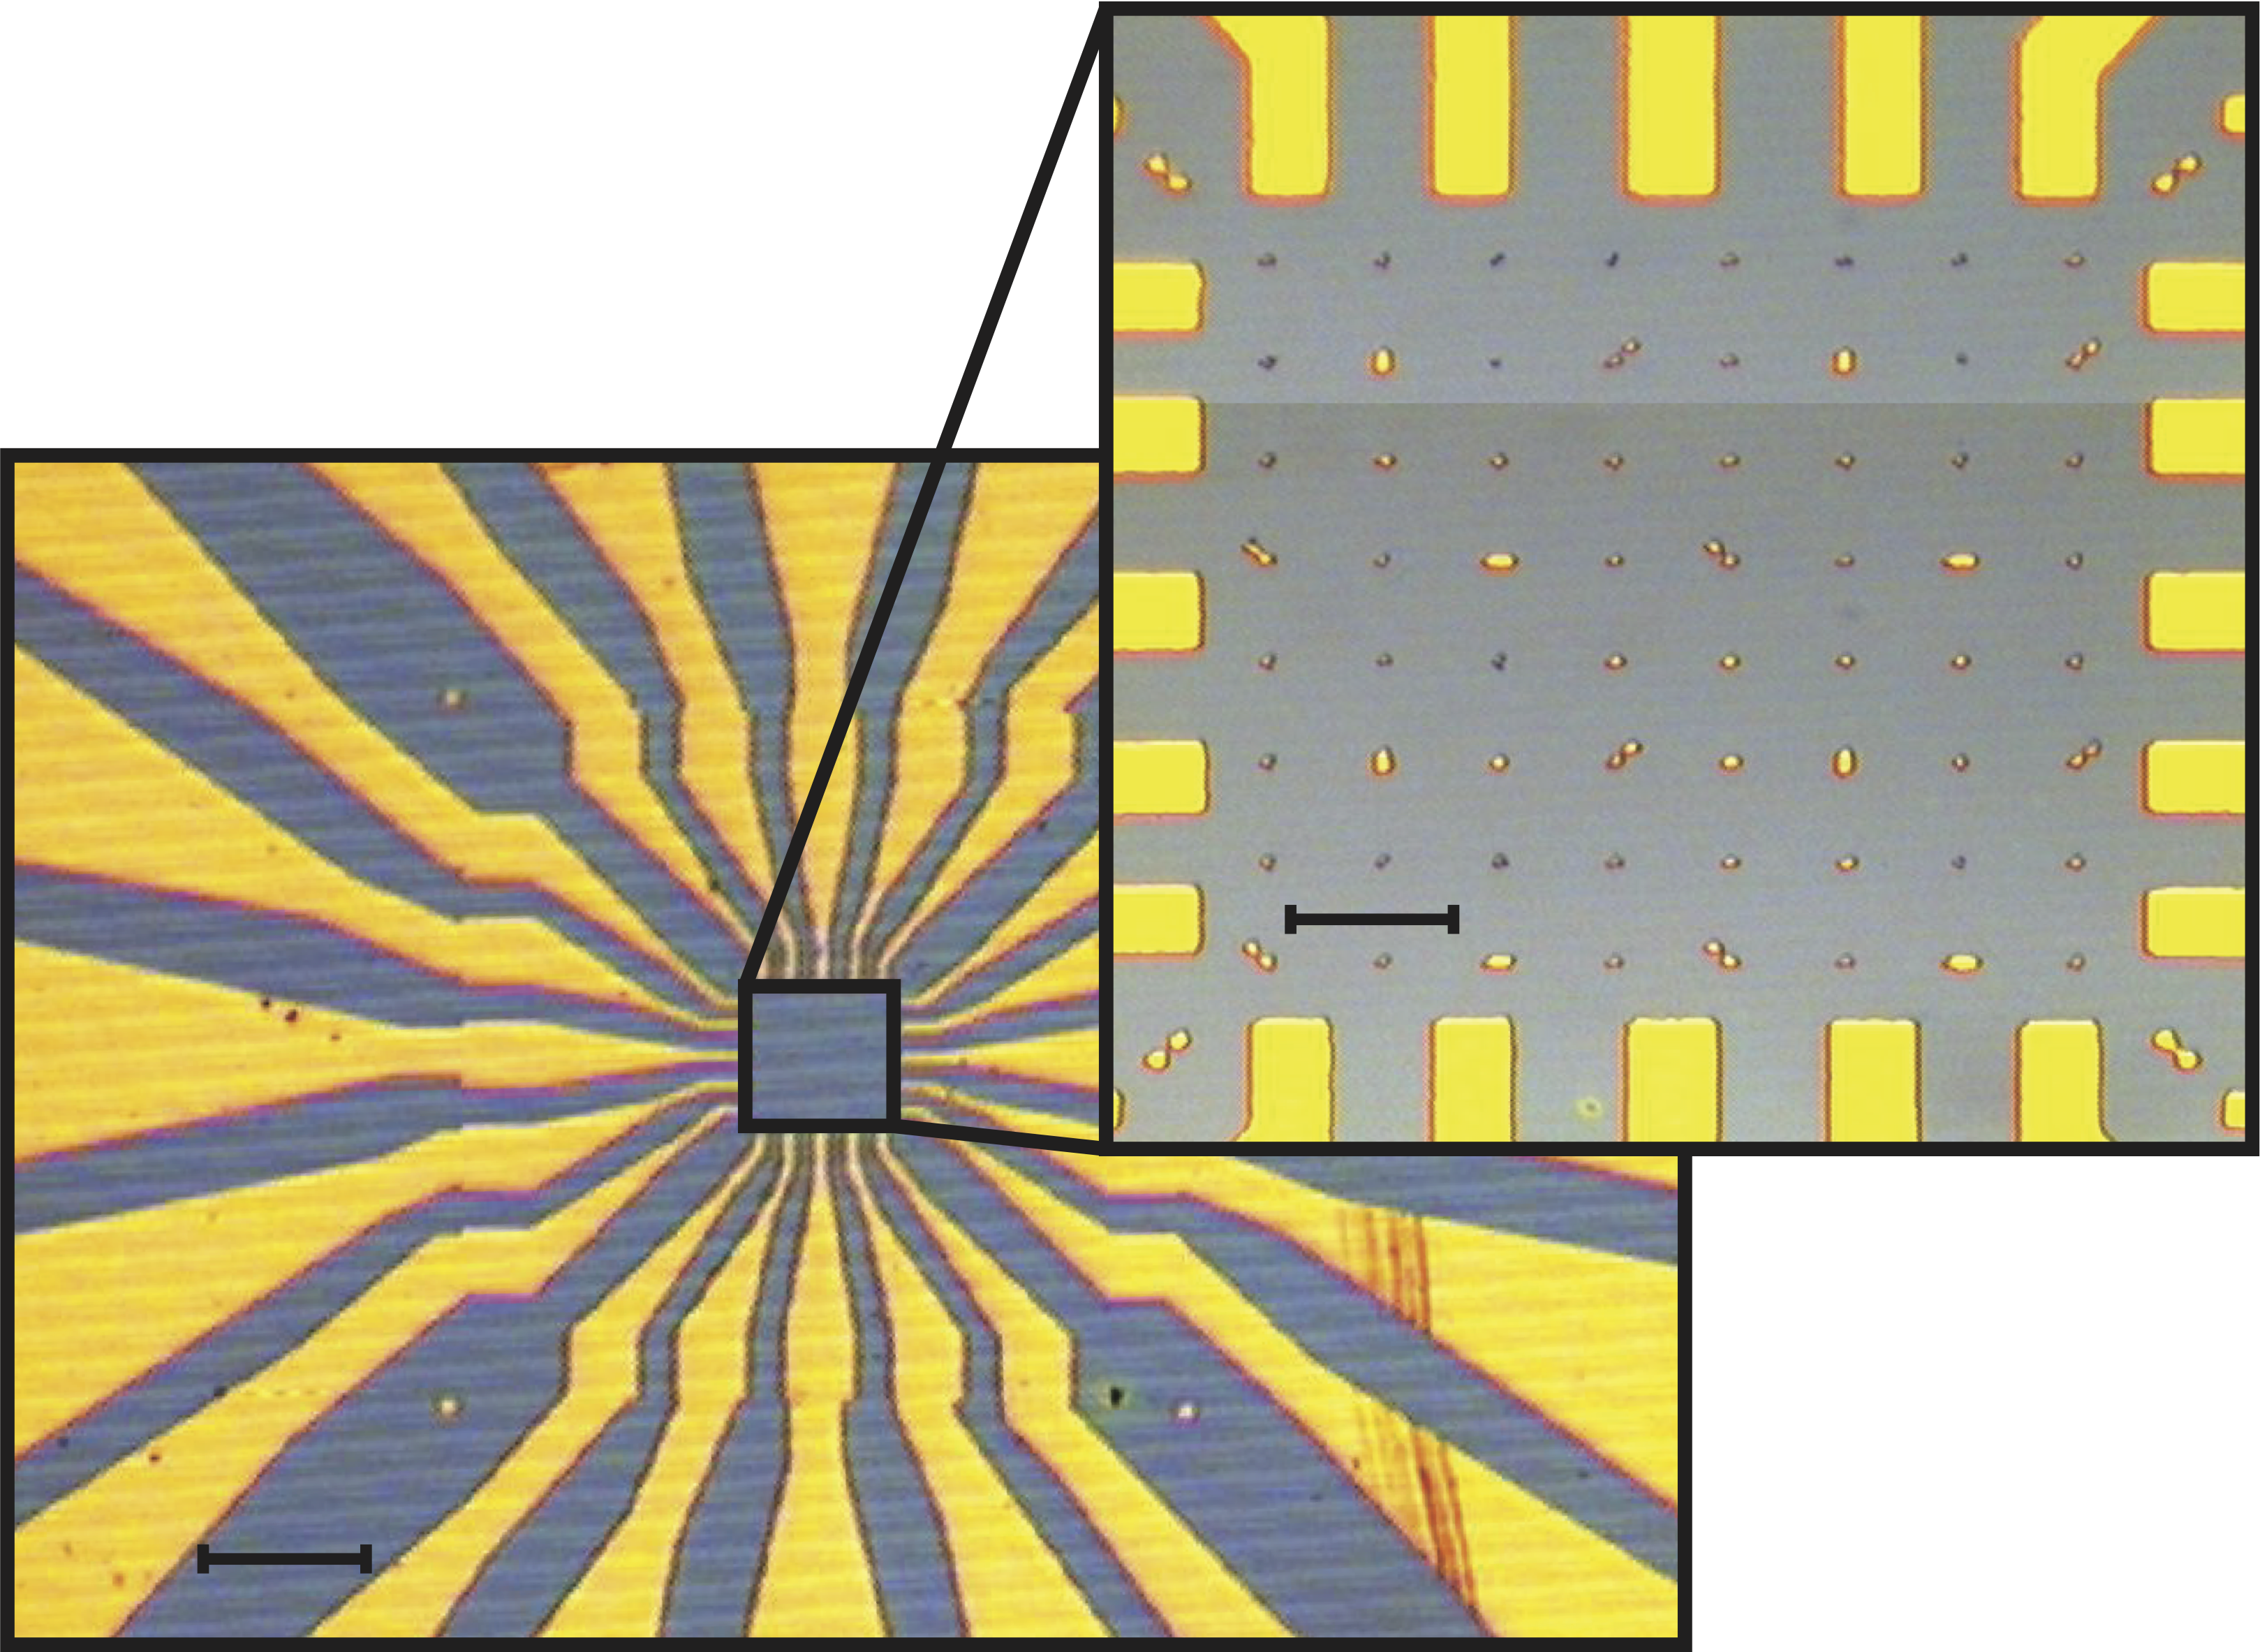
\includegraphics[width = 0.8\textwidth]{chapter3/markers.eps}
    \caption{A \ce{Si}/\ce{SiO2} substrate with \SI{1}{\micro\meter} \ce{Au} markers. Left scale bar: \SI{100}{\micro\meter}. Right scale bar: \SI{20}{\micro\meter} }
    \label{fig:markers}
\end{figure}

\subsection{Advantages and Disadvantages}

Despite having some success fabricating devices using randomly dispersed nanotubes and Electric Force Microscopy scans (Section \ref{subsec:EFM}), the process was found to be too time consuming for frequent use. The main failure point was the preparation of nanotube solutions after growth. The concentrations varied significantly, often producing samples with dense nanotube coverage or no nanotubes found in the regions imaged. Additionally, the process of making a suspended nanotube solution is time consuming. Even those solutions with a useful concentration of nanotubes only remain fully suspended for less than 1 hour. Meaning the process must be repeated frequently.

\section{Catalyst Island Growth}
\label{sec:catalyst_island}

In 1998 \cite{Kong1998a}, it was discovered that the same type of catalyst used to grow nanotubes in powder form (Section \ref{subsec:disperse_catalyst}), could be suspended in solution, patterned, and used to grow nanotubes directly on silicon substrates. When paired with high melting point metals and optical lithography, nanotubes can be grown directly on patterned substrates in known locations. Devices prepared this way take just a fraction of the time to produce. However, these devices were found to be much more prone to other modes of failure, such as leaks in the gate oxide and amorphous carbon contamination on the substrate from the CVD growth process.

\subsection{Catalyst} 

Many different types of catalyst particles can be used in the growth of carbon nanotubes. The ideal catalyst for patterned growth must be compatible with electron beam or optical lithography. Table \ref{table:catalysts} lists most of the catalysts tested in the Markovic lab. To test each catalyst, sputtered molybdenum leads were patterned using the mask aligner and Futurex NR9 resist. Catalyst islands were then patterned using electron beam lithography. Figure \ref{fig:catalyst_islands} shows an example of a substrate with Mo leads and catalyst islands.

\begin{figure}
	\centering
	\includegraphics[width = 0.8\textwidth]{chapter3/catalyst_island.eps}
	\caption{A \ce{Si}/\ce{SiO2} substrate with \SI{3}{\micro\meter} catalyst islands and \ce{Mo} leads. Left scale bar: \SI{100}{\micro\meter}. Right scale bar: \SI{20}{\micro\meter} }
	\label{fig:catalyst_islands}
\end{figure}

\begin{table}
	\centering
	\caption{Patterned Catalysts}
    \begin{tabular}{| r | c || p{70mm} |}
    	\hline
    	\textbf{Catalyst} & \textbf{Suspended In} & \textbf{Results} \\ \hline
        Fe/Mo/alumina \cite{Kong1998} & Methanol & Easy to pattern. Liftoff difficult. Slowly attacks PMMA mask. Appeared to promote gate leaks through the \ce{SiO2} layer. \\ \hline
        Fe/Mo/alumina \cite{Aurich2012} & IPA & Poor adhesion to substrate. \\ \hline
        Fe/Mo/alumina \cite{Ouellette2008} & DI water & Easy to pattern. Excellent adhesion. No gate leak problems. \\ \hline
        \ce{FeCl3} \cite{Hong2005} & DI water & Excellent adhesion to substrate. Not compatible with PMMA mask. Left substrate entirely covered in catalyst. May work well with PDMS stamp. \\ \hline
        thermally evaporated Fe \cite{Biercuk2004, Kang2007} & None & Very easy to pattern. Liftoff is clean. Difficult to control the thickness below \SI{1}{\nano\meter} as required. \\ \hline
    \end{tabular}
    \label{table:catalysts}
\end{table}

All of the devices discussed in this thesis were produced using the Fe\slash Mo\slash alumina catalyst suspended in water. The islands were patterned using electron beam lithography. Catalyst is deposited in the following way:

\begin{enumerate}
	\item Add the powder catalyst from Table \ref{table:powder_catalyst} to \SI{15}{\milli\liter} of DI water and stir for 12 hours
	\item Sonicate the solution for 30 minutes
	\item Cover the sample in catalyst solution for 30 minutes
	\item Dry with \ce{N2} gun
	\item Liftoff by sonicating in acetone for 5 minutes, soaking in a clean acetone for 5 minutes, followed by an isopropanol rinse for 1 minute and a DI water rinse for 1 minute
\end{enumerate}

Obtaining reproducible results in the catalyst deposition was the source of much difficulty. The recipe provided here can be repeated before liftoff shows insufficient catalyst coverage on the substrate. Additionally, it is suspected that baking the catalyst on a hot plate to dry the solution leads directly to gate leaks in the \ce{SiO2} layers and later device failure. Thus, there is no baking step in the deposition of our catalyst islands.

\subsection{Growth}
\label{subsubsec:substrate_cvd}

The recipe for on-substrate growth of nanotubes used in this thesis is very similar to the growth recipe for powder catalyst discussed in Section \ref{subsubsec:powder_cvd}. This recipe was developed over the course of several years from many points of reference \cite{Kong1998, Kong1998a, Dirks2010, Huang2003, Huang2004, Zhang2013, Hong2005} and a my own notes. The recipe is optimized for the 1 inch Lindberg tube furnace as seen in Figures \ref{fig:furnace_setup} and \ref{fig:gas_panel}. Most samples are placed in a smaller \SI{1}{\centi\meter} diameter, 1 foot long quartz tube, then placed in the larger 1 inch diameter quartz tube. This was done to make the samples easier to load into the 1" tube, as well as to reduce turbulence in the gas flow across the sample \cite{Hong2005}. 

The standard nanotube growth recipe used in this work is below:

\begin{enumerate}
	\item Purge the tube by flowing \SI{2000}{\sccm} of Ar for 20 minutes
	\item Heat the tube to \SI{250}{\degreeCelsius} while flowing \SI{300}{\sccm} Ar and \SI{150}{\sccm} \ce{H2}
	\item Wait for at least 1 hour
	\item Heat the tube to \SI{700}{\degreeCelsius} while flowing \SI{300}{\sccm} Ar and \SI{150}{\sccm} \ce{H2}
	\item Wait for 10 minutes
	\item Heat tube to \SI{950}{\degreeCelsius} while flowing \SI{300}{\sccm} Ar and \SI{150}{\sccm} \ce{H2}
	\item Wait for the temperature to stabilize
	\item Flow \SI{700}{\sccm} \ce{CH4} and \SI{150}{\sccm} \ce{H2} for 10-15 minutes
	\item Set temperature to \SI{0}{\degreeCelsius} and let the furnace cool while flowing \SI{300}{\sccm} Ar and \SI{150}{\sccm} \ce{H2}
\end{enumerate}

In almost every case this recipe has grown nanotubes successfully. Steps 2 and 3 are included to remove water vapor from the air that might have collected inside the quartz tube on humid days \cite{Dirks2010}. Steps 4 and 5 are meant to remove iron oxide from the iron nanoparticles that make up the catalyst. 

The most common point of failure has been related to the patterned molybdenum leads on the substrate. Molybdenum oxidizes rapidly at high temperatures. Therefore, any oxygen contamination in the tube during the growth process will form a \ce{MoO} layer that is then quickly removed by reacting with the high temperature \ce{H2} flow. This process repeats and can lead to the Mo leads being entirely etched away. Additionally, it has been found that opening the furnace too soon during cooling can lead to the Mo leads peeling off of the substrate. This appears to be caused by some super-heating due to IR radiation reflecting off of the surfaces of the sample and quartz tube. It is a strange phenomenon that is avoided by allowing the furnace to cool to less than \SI{300}{\degreeCelsius} before opening the lid. These problems could also be solved by using a different high temperature metal such as a W/Pt bilayer, common in many other nanotube projects. Molybdenum was chosen for this work because it is easy to sputter and much more affordable.

\subsection{Advantages and Disadvantages}

Growing nanotubes from catalyst islands near predefined leads and markers offers a large improvement in processing time over the method of random dispersion. Nanotubes produced with this method are longer, cleaner, and easier to locate. These improvements made this method the obvious choice for device fabrication. The disadvantages stemming from substrate contamination during growth or imaging can be overcome by simply increasing number of samples produced.

\section{Imaging Nanotubes}
\label{subsubsec:imaging_disperse}

Nanotubes on a \ce{SiO2} surface can be located in a number of ways. This section will review a number of different methods, focusing on improvements made in the course of this thesis work.

\subsection{Atomic Force Microscopy}

With nanotubes that have been drop cast onto the surface, the standard method is to locate the tubes relative to the predefined markers using a tapping mode atomic force microscope (AFM). An example of an image created this way is seen in Figure \ref{fig:cnt_au_markers}. 

\begin{figure}
	\centering
	\includegraphics[width = 0.8\textwidth]{chapter3/cnt_au_markers.png}
	\caption{A composite image made from several AFM height measurements of a sample with nanotubes dispersed over a  substrate with \SI{1.5}{\micro\meter} gold markers. The scale bar is \SI{10}{\micro\meter}.}
	\label{fig:cnt_au_markers}
\end{figure}

This method is very reliable, but extremely time consuming. In order to resolve nanotubes, as well as the predefined markers in the image, AFM scan sizes must be limited to \SI{25}{\square\micro\meter}. Each of these scans takes 30 minutes and many scans are needed to fully image one patterned substrate. Looking closely at Figure \ref{fig:cnt_au_markers}, there are 12 scans covering less than half the substrate. Due to vibrational noise and piezo limits, some images are slightly warped. Stitching the images together is time consuming and inaccurate.

\subsection{Electric Force Microscopy}
\label{subsec:EFM}

The Digital Instruments Nanoscope 3 used in our lab is also capable of making electric force microscope (EFM) measurements. An EFM image is made by first measuring the height across the sample in standard tapping mode, then using that height data to run a second 'interleave' scan at a fixed height with a bias voltage applied between the tip and sample. By holding the tip at a fixed height, van der Waals interactions between the tip and sample are constant and the only force measured is the electrostatic force from the applied bias voltage. Contrast in the resulting images is related to the different conductivities of the objects on the sample \cite{Bockrath2002}. Thus, conducting (and semiconducting) nanotubes have a high contrast against the insulating \ce{SiO2} substrate. An example of this type of image is shown in Figure \ref{fig:cnt_efm}

\begin{figure}
	\centering
	\includegraphics[width = 0.8\textwidth]{chapter3/cnt_efm.eps}
	\caption{An EFM image of nanotubes dispersed over a substrate with \SI{1.5}{\micro\meter} gold markers. The markers have been automatically located using the height data and highlighted in blue on the EFM image. The scale bar is \SI{10}{\micro\meter}.}
	\label{fig:cnt_efm}
\end{figure}

An entire patterned substrate can be scanned using this method in about 1 hour. The scan size can be increased up to \SI{75}{\square\micro\meter} due to the false contrast provided by the large electrostatic forces between the nanotubes and the tip. Rather than appearing as \SI{1}{\nano\meter} in diameter, the tubes appear in the EFM image to be about 100 times their real diameter. This was a notable improvement over locating nanotubes using AFM height scans alone. Comparing Figure \ref{fig:cnt_au_markers} and Figure \ref{fig:cnt_efm}, it is clear the EFM image is far more useful in locating nanotubes.

\subsection{EFM Through PMMA}

All of the same techniques from Section \ref{subsubsec:imaging_disperse} can be applied to imaging nanotubes grown from patterned catalyst islands. However, because the substrates are not covered in closely spaced markers, it was found that tapping mode AFM height scans were not useful. Scans could only cover a small part of the sample and the resulting images were difficult to orient.

Using electric force microscopy (EFM) made it possible to scan the entire region of interest on the sample in one measurement. An example of this type of scan is shown in Figure \ref{fig:efm_islands}a. As can be seen in that figure, it was difficult for the AFM tip to avoid crashing into the catalyst islands during the EFM sweep. The catalyst islands are several hundred nanometers in height while the other features on the substrate are less than \SI{10}{\nano\meter}. Such height differences make large area scans difficult in tapping mode. This problem can be avoided by coating the sample in PMMA before scanning with the EFM, as seen in Figure \ref{fig:efm_islands}b. The PMMA coating smooths the height differences between the substrate and catalyst islands, without compromising the contrast between the insulating substrate and conducting nanotubes. The idea was adopted from a 2007 paper in which the authors attempted to locate nanotubes suspended in a PMMA layer in three dimensions \cite{Jespersen2007}.

\begin{figure}
	\centering
	\includegraphics[width = 1.0\textwidth]{chapter3/efm_islands.eps}
	\caption{(a) Frequency data collected from an EFM scan of a catalyst island sample after nanotube growth. (b) Frequency data collected from an EFM scan of a similar sample. Prior to the scan this sample was coated with a \SI{250}{\nano\meter} PMMA layer. Both scale bars are \SI{10}{\micro\meter}. }
	\label{fig:efm_islands}
\end{figure}

\subsection{Scanning Electron Microscopy}
\label{subsec:imaging_sem}

In 2002, a paper \cite{Brintlinger2002} was published illustrating that a scanning electron microscope (SEM), operating at a low accelerating potential could provide a similar type of false contrast image as produced by the EFM. The insulating substrate tends to collect charge from the electron beam, while the conducting nanotubes do not. This produces an image in which the nanotubes appear as bright lines about 100 times their actual diameter. An example of this is seen in Figure \ref{fig:sem_islands}. 

\begin{figure}
	\centering
	\includegraphics[width = 0.8\textwidth]{chapter3/sem_islands.eps}
	\caption{A scanning electron micrograph of a catalyst island sample after nanotube growth. The scale bar is \SI{10}{\micro\meter}.}
	\label{fig:sem_islands}
\end{figure}

Typically, an EFM scan of a sample will take 45 minutes. A SEM image of the same sample takes less than 2 minutes. However, the SEM can introduce some carbon contamination from the high energy electrons passing through small amounts of oil mist back-streaming into the vacuum chamber from the mechanical roughing pump. Due to the large number of samples that were produced to obtain the data in this thesis, it was decided that contamination from the SEM was an acceptable risk, given the immense time savings.

\section{Image Filtering}

Once it became clear that the scanning electron microscope was by far the most efficient and reliable way to locate carbon nanotubes on a substrate, it also became important to optimize those images to revel the most information possible. The resolution and contrast in the SEM images produced in our lab are limited by the the use of a thermionic \ce{LaB6} filament. Unlike field emission scanning electron microscopes, which are more common in nanofabrication, the thermionic scanning electron microscope has a large initial crossover size, requiring more electromagntic lens focusing to produce a sufficiently small beam size for imaging. This problem is exasperated when using low accelerating potentials (500-\SI{3000}{\volt}), which are crucial to achieving good contrast of carbon nanotubes on a silicon substrate.

\subsection{Histogram Equalization}

This method was based on two corrections. First, a plane fit to correct for the position of the secondary electron detector. Second, finding the histogram then transforming it such that there are equal numbers of pixels at each brightness level. An illustration of this can be seen in Figure \ref{fig:hist_eq}

\begin{figure}
	\centering
	\includegraphics[width = 0.4\textwidth]{chapter3/histogram_equalization_wiki.png}
	\caption{An illustration of the histogram equalization process.}
	\label{fig:hist_eq}
\end{figure}

Figure \ref{fig:hist_eq_data} shows the process of filtering an SEM image using histogram equalization. At the top of figure is the original image after a plane fit (to correct changes in brightness across the substrate). To the right of the image, the histogram of brightness values and the cummulative distribution function are plotted. The center image is after the histogram equalization. Contrast is now dramatically increased in the image, the histogram is nearly flat, and the cumulative distribution function is linear. Finally, the image is gaussian filtered using a $3 \times 3$ kernel to reduce the high frequency noise, which has been exaggerated by the histogram equalization. The final histogram is not flat quite flat and the cumulative distribution function is not quite linear. However, the contrast in the image has been enhanced significantly

\begin{figure}
	\centering
	\includegraphics[width = 0.8\textwidth]{chapter3/histogram_eq_example.pdf}
	\caption{Top image is the original SEM image after a plane fit. Middle image shows the SEM image after histogram equalization. Bottom image shows the final result after gaussian smoothing. Plots on the right show the histogram of brightness values and cumulative distribution function at each step.}
	\label{fig:hist_eq_data}
\end{figure}

While this filter does succeed in increasing contrast in the image, which was the main problem associated with our SEM, it also increases the background noise to often unacceptable levels. Histogram equalization does not use any specific information about the carbon nanotubes and substrates being imaged. A better filter should be possible by taking advantage of the fact that the features of interest can be well characterized in a sample set of images. 

\subsection{Matched Filter Bank}

Matched filter banks are a well known technique that have been used very successfully to filter retinal images in medicine \cite{Chaudhuri1989}. This technique has previously been adapted to high resolution SEM images of carbon nanotube bundles \cite{Guerrero2014}. The following section describes the implementation of this method to filter images of single walled carbon nanotubes grown on insulating substrates. 
%% nanotube profiles -> kernel -> filtering/thresholding

\subsubsection{Nanotube Profile Model}

To begin building the matched filter bank, the profile shape of a single nanotube from the SEM image must be determined. To find this shape, a random set of 25 SEM images was selected (similar to those in Figure \ref{fig:sem_islands}). From each of these images, images of two nanotubes were cropped. Those nanobues can be seen in Figure \ref{fig:all_nanotube_sections}a. Each of these images was then rotated such that the longest straight portion (that could be identified by eye) was oriented vertically. The profile of the nanotube was averaged over that long straight section. These results are plotted in Figure \ref{fig:all_nanotube_sections}b.

\begin{figure}
	\centering
	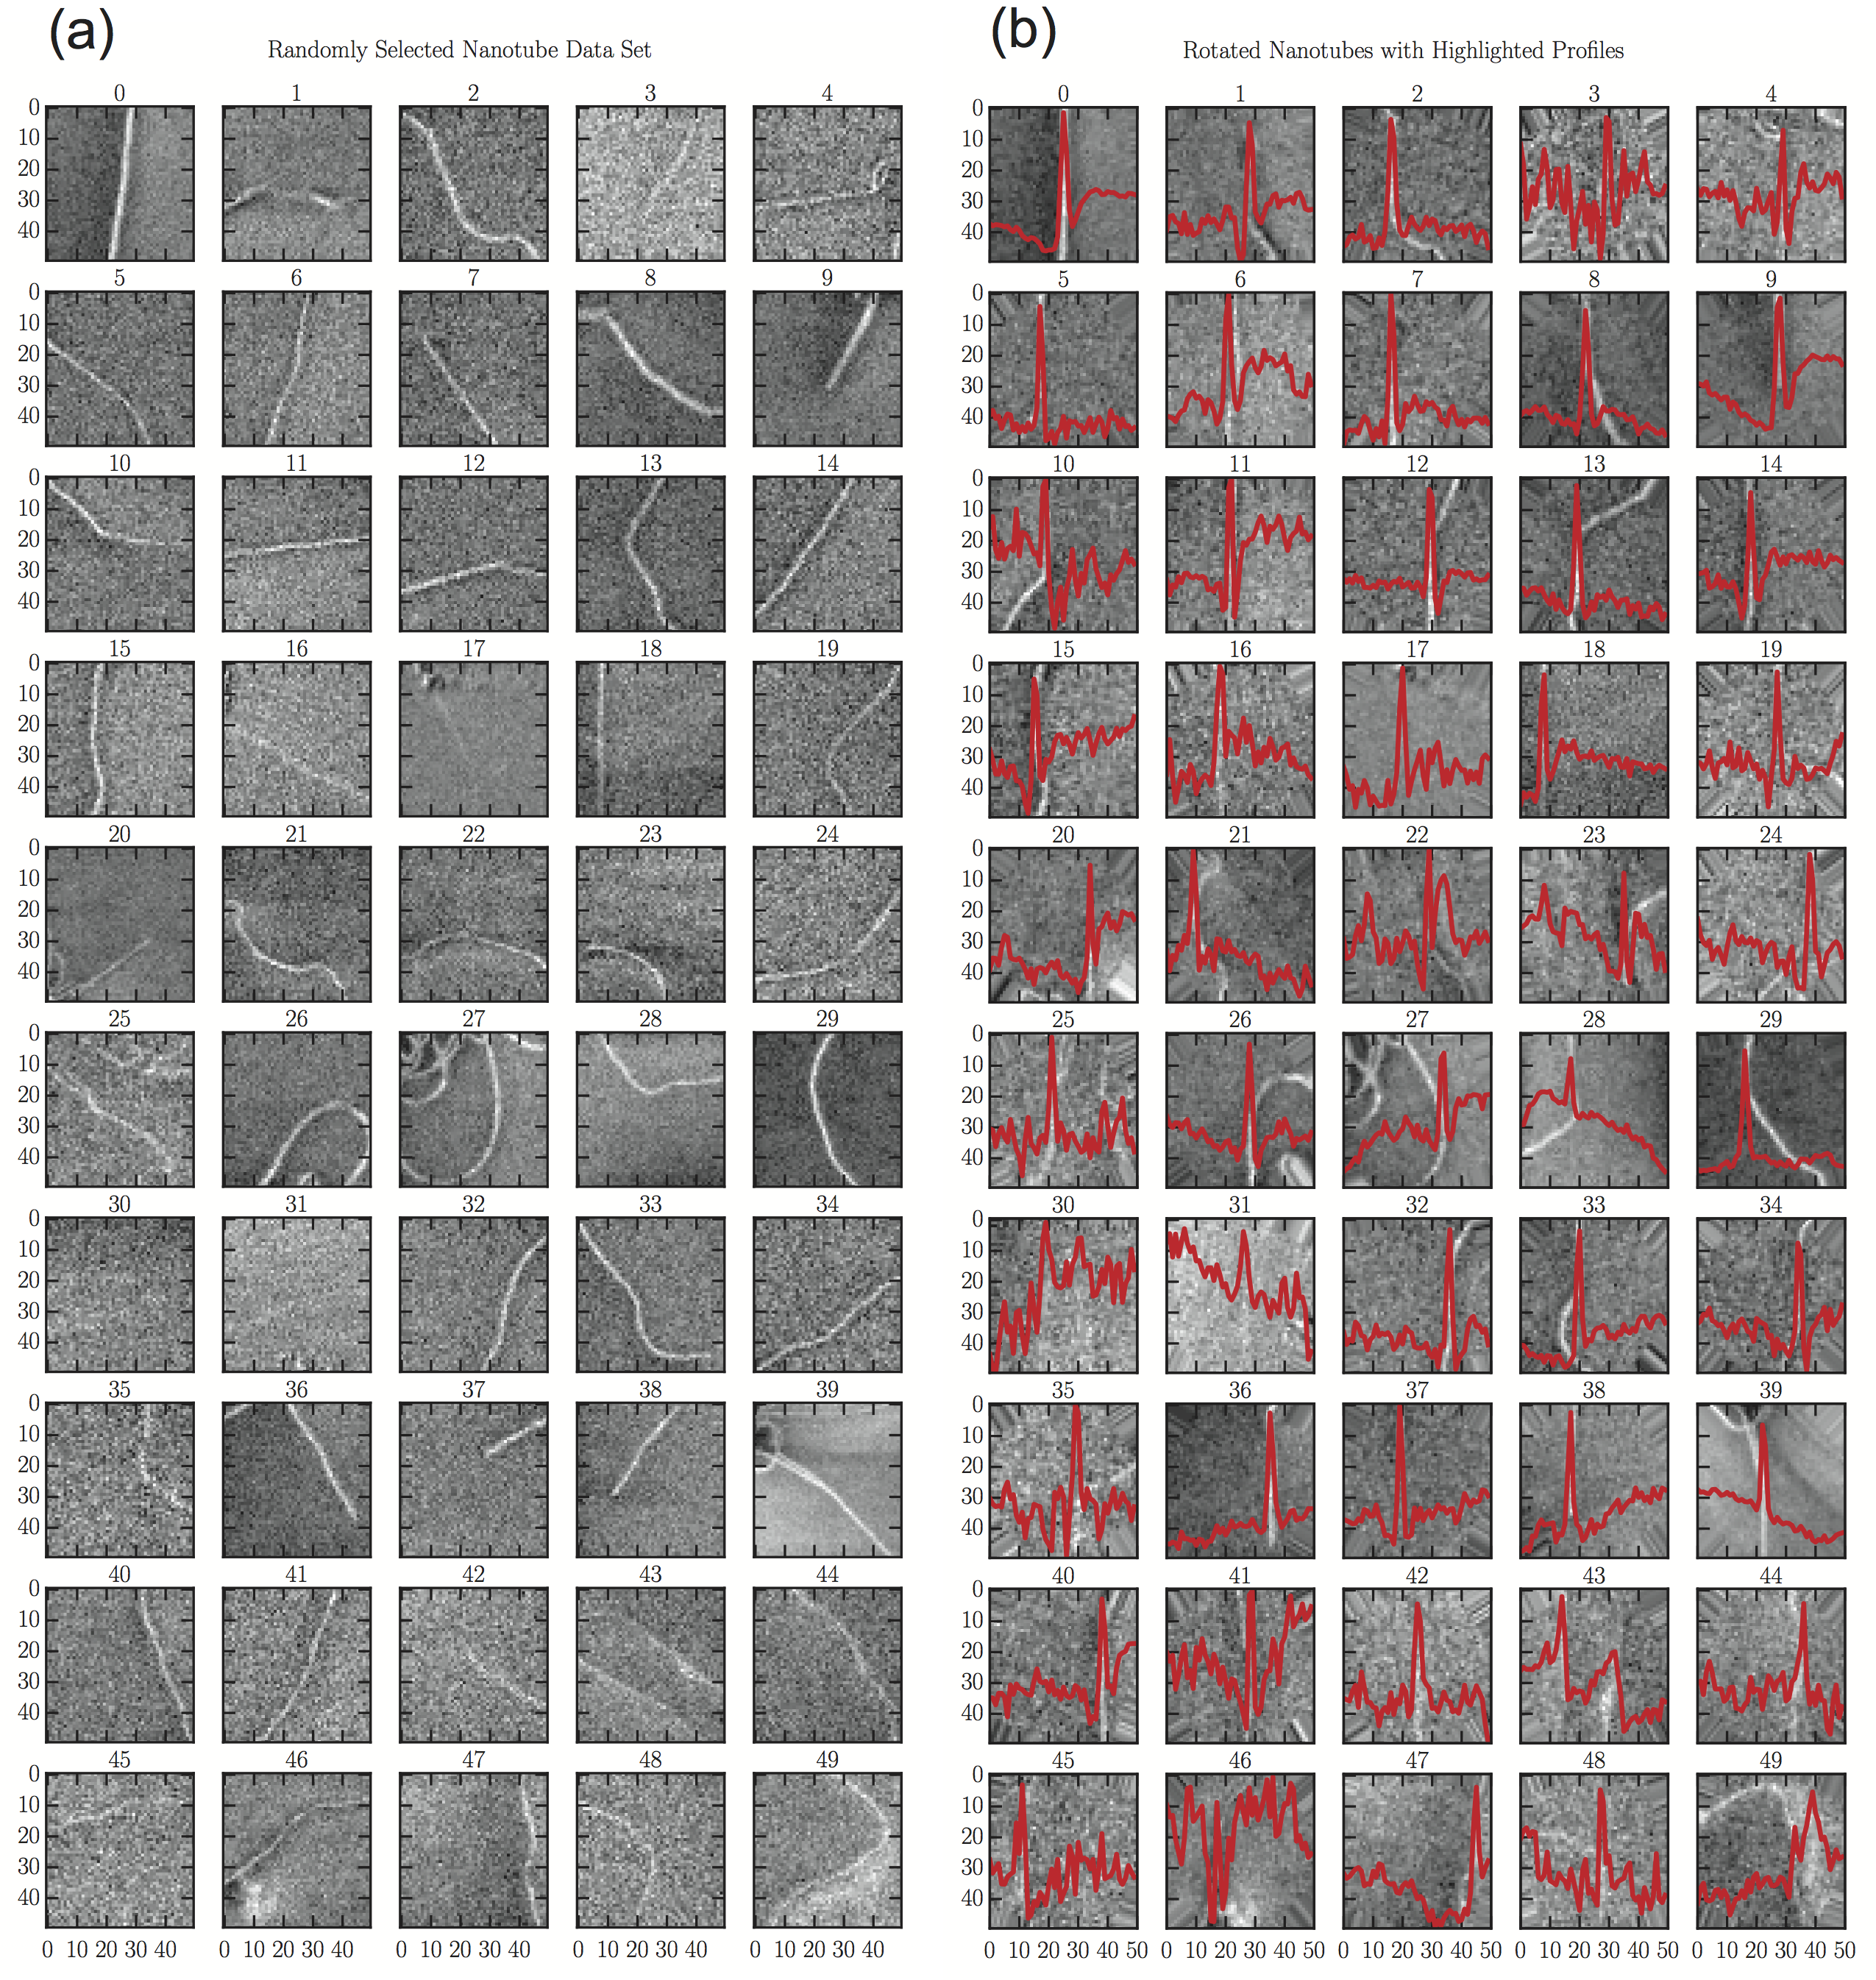
\includegraphics[width = 1.0\textwidth]{chapter3/all_nanotube_sections.eps}
	\caption{a) The original data set of SEM nanotube images used to create and optimize the matched filter bank. b) The same data set rotated and overlaid with extracted nanotube profiles.}
	\label{fig:all_nanotube_sections}
\end{figure}

Based on the shape of these profiles a truncated $sinc$ function, Equation \ref{eq:sinc}, was chosen to fit the nanotube profile.

\begin{equation} 
\label{eq:sinc}
    f(x) = \begin{cases} \frac{A\sin{kx}}{kx} & |x| < \frac{2\pi}{k} \\ 
                         0                    & |x| > \frac{2\pi}{k} 
           \end{cases}
\end{equation}

This fuction was chosen because it captures the bright nanotube peak and dark regions beside the nanotube while still only requiring one fit parameter. To determine the fit parameters the linear background was subtracted from each profile in Figure \ref{fig:all_nanotube_sections}b and the profiles were  fit using \ref{eq:sinc}. The results of this fitting can be seen in Figures \ref{fig:profile_fits}a and b. 

\begin{figure}
	\centering
	\includegraphics[width = 1.0\textwidth]{chapter3/profile_fits.eps}
	\caption{a) Extracted nanotube profiles with linear background removed (blue). Fits to \ref{eq:sinc} (red). b) Distribution of $k$ values extracted from profile fits. c) Distribution of straight nanotube section lengths.}
	\label{fig:profile_fits}
\end{figure}

\subsubsection{Filter Kernel}

The filter kernel is built starting with the median $k$ value found from the profile fits. To extract each profile, horizontal cuts of the nanotube image were averaged over a straight segment of the nanotube that was identified and labelled by hand. The distribution of these straight segment lengths can be seen in Figure \ref{fig:profile_fits}c. Again, to proceed with building the filter we use the median value of $L$ from that distribution. The kernel is built in an $N \times N$ matrix with $(x,y) = (0,0)$ at the center of the matrix. The full kernel, $K(x,y)$ is defined by Equation \ref{eq:kernel}.

\begin{equation} 
\label{eq:kernel}
K(x,y) = \begin{cases} \frac{A\sin{kx}}{kx} & |x| < \frac{2\pi}{k}, |y| < \frac{L}{2} \\ 
                       0                    & |x| > \frac{2\pi}{k},  |y| > \frac{L}{2}
       \end{cases}
\end{equation}

Once the kernel is defined on the $N \times N$ matrix, the kernel is normalized such that the sum over all of the matrix elements is equal to zero. By convolving this kernel with the SEM image, portions of the image with a shape matching the fit profile and a length $L$ will highlighted in the output. This results in significant background subtraction and accurate nanotube enhancement. 

\subsubsection{Filter Bank}

To build the full filter bank, the kernel, built using Equation \ref{eq:kernel}, is rotated by a set of angles between $0$ and $\pi$. Each of these filters is then convolved with the image separately. By doing this, it is possible to identify nanotube sections lying along any direction on the substrate. A binary result is created using thresholding on the convolved image. The filter bank and resulting binary images can be seen in Figures \ref{fig:filter_bank_results}c and d. 

\begin{figure}
	\centering
	\includegraphics[width = 0.8\textwidth]{chapter3/filter_bank_results.eps}
	\caption{a) Original image. b) Final filtered image, which is the sum of the binary images in (d). c) The rotated kernels that form the full matched filter bank. d) Each rotated kernel applied to an image in (a).}
	\label{fig:filter_bank_results}
\end{figure}

After each kernel has been separately convolved with the original image, and the threshold applied, those binary images are added together to produce the final filtered image. Figures \ref{fig:filter_bank_results}a and b show the original and filtered nanotube images. 

In building this filter, many parameters had to be optimized simultaneously and compared by eye. Due to the large parameter space, the matched filters were optimized by iteratively varying a single parameter and choosing the best result. This process is illustrated in Figure \ref{fig:filter_parameter_test}.

\begin{figure}
	\centering
	\includegraphics[width = 0.7\textwidth]{chapter3/filter_parameter_test.pdf}
	\caption{Optimization of the matched filter bank threshold value.}
	\label{fig:filter_parameter_test}
\end{figure}

The results of this optimization are seen in Table \ref{table:filter_parameters}. The optimized values for $k$ and $L$ were very close to those obtained from the original analysis of extracted nanotube profiles. Note that $A$ and $threshold$ are not independent values and $A$ remained fixed for this optimization procedure. 

It is also important to note that the length scale for these parameters is in pixels $(px)$. The randomly selected SEM images that were used for this analysis were not all take at the same magnification level. However, the average magnification was $850\times$ giving a pixel size of $\sim$\SI{140}{\nano\meter}

\begin{table}
	\centering
	\caption{Matched Filter Bank Parameters}
	%\hfill \\
    \begin{tabular}{| r | p{60mm} | l |}
    	\hline
    	\textbf{Parameter} & \textbf{Description} & \textbf{Optimized Value}  \\ \hline
    	k & inverse length scale for $sinc$ fit &  $1.75 px^{-1}$ \\ \hline
    	A & height of $sinc$ function in $K(x,y)$ &  $10$ \\ \hline
    	L & length of straight nanotube sections to search for &  $16 px$ \\ \hline
    	N & size of the kernel matrix &  $25$ \\ \hline
        R & number of kernels in the filter & $15$ \\ \hline
        threshold & cutoff value for thresholding images convolved with filter kernels & $3.6$ \\ \hline
    \end{tabular}
    \label{table:filter_parameters}
\end{table}

Finally, the filter was tested with the original set of full device SEM images. A selection of the results can be seen in Figure \ref{fig:full_image_filter}. It is clear from this set of images that the filter has the desired result. Nanotubes are much more clearly visible and the background is almost completely removed. Because the filter is very similar in its construction to common edge detection algorithms, it also leaves features at the edges of the optical lithography leads and markers defined on the substrate before nanotube growth. This actually works well, since those features are used to align the SEM images for additional electron beam lithography steps. 

\begin{figure}
	\centering
	\includegraphics[width = 1.0\textwidth]{chapter3/full_image_filter_test.pdf}
	\caption{Optimization of the matched filter bank threshold value.}
	\label{fig:full_image_filter}
\end{figure} % growth of CNT, placement on substrate, imaging
\chapter{Metallic Contacts to Carbon Nanotubes}
\label{sec:contacts}
\chaptermark{Contacts to CNTs}

Chapter will contain: an explanation of the nature of metal-nanotube interfaces, statistics on metals tested, thin film deposition methods, and lithography methods. opinions will be backed up with a lot of histograms, contact resistance data, and device images. It's not the most exciting chapter, but it is what I spent a great deal of time thinking about over the past two years. %barrier info, statistics on lithography/deposition methods
\chapter{Quantum Dots with Ferromagnetic Leads}
\label{sec:FMCNTQD}
\chaptermark{Ferromagnetic CNTQD}

Of the many samples discussed in Chapter \ref{chap:contacts}, seven FM-CNT-FM devices were measured at low temperatures. Details, including room temperature resistance, can be seen in Table \ref{table:rt_fm_devices}.

\begin{table}
    \centering
    \begin{tabular}{ r | c | c c c}
        Sample & Leads & Material & Deposition Method & R($T=300K$) \\ \hline
        SCF72 & 17-19 & Co & sputter & \SI{65}{\kilo\ohm} \\
        SCF72 & 21-23 & Co & sputter & \SI{76}{\kilo\ohm}\\
        SCF75 & 21-23 & Co & sputter & \SI{280}{\kilo\ohm}\\
        SCF75 & 15-16 & Co & sputter & \SI{30}{\kilo\ohm}\\
        SCF96 & 9-12  & Co & electron beam evaporation & \SI{200}{\kilo\ohm}\\
        SCF96 & 16-17 & Co & electron beam evaporation & \SI{400}{\kilo\ohm}\\
        SCF98 & 11-12 & Co & electron beam evaporation & \SI{120}{\kilo\ohm}\\
        \label{table:rt_fm_devices}  
    \end{tabular}
    \caption{Details of measured FM-CNT-FM devices}
\end{table}

Each of these samples was measured at 4K, with the exception of SCF98 (11-12) which was measured at 150mK. Figure \ref{fig:all_FM_QD} shows Coulomb diamond plots for each of the samples. These were used to calculate the quantum dot properties seen in Table \ref{table:cold_fm_devices}

\begin{table}
    \centering
    \footnotesize
    \begin{tabular}{ r | r | c c c c c c c}
        Sample & Leads & $\Delta \mu (meV)$ & $\Delta E (meV)$ & $\frac{e^2}{2C} (meV)$ & $L_{measured} (nm)$ & $L_{design}$ (nm) & $C_{\Sigma} (aF)$ & $\alpha_{G}$ \\ \hline
        SCF72 & 23-21 & 8  & x   & x    & 175 & 300 & x  & 0.080 \\ 
        SCF72 & 17-19 & 8  & 1.8 & 6.2  & 280 & 300 & 13 & 0.072 \\
        SCF75 & 21-23 & 15 & 4.5 & 11.5 & 110 & 300 & 7  & 0.075 \\
        SCF75 & 15-16 & 12 & 3.5 & 8.5  & 140 & 300 & 9  & 0.110 \\
        SCF96 & 9-12  & 30 & 4.0 & 26.0 & 125 & 300 & 3  & 0.011 \\
        SCF96 & 16-17 & 22 & 2.0 & 20.0 & 250 & 300 & 4  & 0.006 \\
        SCF98 & 11-12 & 7  & 1.8 & 5.2  & 280 & 300 & 15 & 0.005 \\
        \label{table:cold_fm_devices}  
    \end{tabular}
    \caption{Low temperature characteristics of FM-CNT-FM quantum dots}
\end{table}

\begin{figure}
    \centering
    \includegraphics[width=1.0\textwidth]{fmdots/all_fm_dots.png}
    \caption{Conductance as a function of $V_{bias}$ and $V_{gate}$ for all measured ferromagnetic quantum dots.}
    \label{fig:all_FM_QD}
\end{figure}

The lever arm, $\alpha_{G}$, defined as $\alpha_{G} = C_G/C_{\Sigma}$ and is used to convert gate voltages to energies, $U_{gate} = \alpha_{G}eV_{gate}$ \cite{Ihn2004}. The lever arm can be calculated based on the geometry of the Coulomb diamonds. Figure \ref{fig:alpha_calc} illustrates how to calculate $\alpha_{G}$. The lever arm characterizes the coupling regime for each devices. Looking at the lever arm values, the electron beam evaporated samples are in a much weaker coupling regime than the sputtered samples. All other aspects of the fabrication were the same over all four samples. 

\begin{figure}
    \centering
    \includegraphics[width=0.6\textwidth]{fmdots/alpha_calc.pdf}
    \caption{Calculating the lever arm using Coulomb diamond geometry.}
    \label{fig:alpha_calc}
\end{figure}

\section{Tunneling Magnetoresistance}

Tunneling magnetoresistance is an change in resistance measured across a ferromagnet/insulator/ferromagnet structure. The spin transport through such an interface can be made tunable by replacing the insulator with a carbon nanotube quantum dot. Exchange coupling with the ferromagnetic leads will split the spin degeneracy of the quantum dot, making it possible to tune the magnitude and even the sign of the tunneling magnetoresistance \cite{Tsymbal2003, Sahoo2005, Thamankar2006}.

The magnetization of the carbon nanotube contacts is dominated by their shape anisotropy. This is typical for polycrystaline sputtered and electron beam evaporated films, such as the ones used in these samples. By patterning the contacts with different widths, they have different coercive fields at which the magnetization will be flipped as an external, parallel magnetic field is varied. A schematic of the situation can be seen in Figure \ref{fig:spin_valve}.

\begin{figure}
    \centering
    \includegraphics[width=0.9\textwidth]{fmdots/TMR.pdf}
    \caption{Top: A diagram of the magnetization of the ferromagnetic nanotube contacts corresponding to the data shown in the lower plot. Bottom: TMR signal measured through a carbon nanotube quantum dot.}
    \label{fig:spin_valve}
\end{figure}

\subsection{Results}

Of the ferromagnetic devices measured, only sample SCF72 showed clear tunneling magnetoresistance behavior. Refer to the previous section for details on that sample. In the other devices the effect was overwhelmed by random telegraph noise in the data, which can look a lot like false TMR signals, or the metal/nanotube barriers had impurities that caused spin flipping events that destroyed the TMR effect.

\begin{figure}
    \centering
    \includegraphics[width=0.9\textwidth]{fmdots/scf72_17-19_TMR_4K.pdf}
    \caption{Tunneling magnetoresistance measurements taken on device SCFM72 (17-19) at $V_{gate} = 0V$. The plots show data for $V_{bias} = 5mV$ (left) and $V_{bias} = 10mV$ (right).}
    \label{fig:TMR_real}
\end{figure}

In the simplest mode, tunneling magnetoresistance is defined as:

\begin{align}
    TMR \equiv \frac{G_P - G_{AP}}{G_P + G_{AP}} = \frac{R_{AP} - R_{P}}{R_P + R_{AP}} \\
    TMR = P_L P_R \label{eq:basic_tmr}
\end{align}

Where $P_{L(R)}$ are the spin polarizations at the Fermi level for the left and right nanotube contacts \cite{Maekawa1982}. This polarization is defined as:

\begin{equation}
    P_{L(R)} = \frac{\rho^{L(R)}_{+} - \rho^{L(R)}_{-}}{\rho^{L(R)}_{+} + \rho^{L(R)}_{-}}
\end{equation}

And $\rho^{L(R)}_{+(-)}$ are the tunneling density of states for the majority (minority) spins at the Fermi level. With all of this one expects that $P_{L(R)}$ will be positive, thus the TMR signal will be positive.

In the data shown in Figure \ref{fig:TMR_real}, the TMR signal is measured to be about -6.0\% and -0.8\% in the left and right plots, respectively. Additionally, the coercive fields for the two cobalt contacts are bout 40mT and 60mT. These coercive field measurements are consistent with the predicted values for narrow cobalt wires.

The TMR signal has a magnitude consistent with the predicted values \cite{Maekawa1982}, but with the opposite sign. This change in sign of the TMR signal has previously been explained by a resonant tunneling model with asymmetric coupling of the left and right contacts to the nanotube. The model as described here is taken from \cite{Tsymbal2003}.

First the conductance through the quantum dot can be written as:

\begin{equation}
\label{eq:tunnel_conductance}
    G(E) = \frac{4e^2}{h} \frac{\Gamma_L \Gamma_R}{(E-E_i)^2 + (\Gamma_L + \Gamma_R)^2}
\end{equation}

Here, $\Gamma_{L(R)}$ are the tunneling rates on/off the quantum dot from the left(right) ferromagnetic contacts. These tunneling rates can be thought of as being proportional to the density of states of the on the leads. $E_i$ is the energy of the quantum dot level nearest to the Fermi level of the leads $E$. 

When the quantum dot is tuned off resonance $|E-E_i| \gg \Gamma_L + \Gamma_R$ and the TMR signal is predicted by Equation \ref{eq:basic_tmr}. Near a resonant level, $E \sim E_i$ the situation is quite different. Considering the limit where $\Gamma_L \gg \Gamma_R$, Equation \ref{eq:tunnel_conductance} simplifies to $G \sim \frac{\Gamma_R}{\Gamma_L}$. The conductance is now inversely proportional to the density of states on one of the leads, which leads to a sign inversion of the TMR signal.

\begin{equation}
\label{eq:sign_inversion}
    TMR = -P_L P_R
\end{equation}

By using a carbon nanotube quantum dot, the TMR signal can be modulated by tunning the resonant energy level $E_i$ with the gate voltage. Additionally, the magnitude can be modulated because the levels on the quantum dot are spin non-degenerate due to the exchange coupling field introduced by the magnetic leads. This effect has been observed previously in carbon nanotube quantum dots \cite{Sahoo2005, Thamankar2006}. 

In sample SCF72, the TMR signal was only significant in a narrow range of gate voltages near $V_{gate}=0V$, as shown in Figure \ref{fig:TMR_real}. Looking at the conductance data as a function of the gate voltage in Figure \ref{fig:TMR_gate}, it is clear that at $V_{gate}=0V$ there is a quantum dot level $E_i$ resonant with the Fermi level on the leads. Therefore, the observed negative TMR signal makes sense in terms of the model described.

\begin{figure}
    \centering
    \includegraphics[width=0.9\textwidth]{fmdots/scf72_17-19_gateswp-for-TMR.pdf}
    \caption{Conductance as a function of $V_{gate}$ for sample SCF72. Note the conductance peak at $V_{gate}=0V$.}
    \label{fig:TMR_gate}
\end{figure}

%%%%%%%%%%%%%%%%

%\section{Magnetoresistance with Non-Colinear Ferromagnetic Leads}
%
%Maybe later

%%%%%%%%%%%%%%%%

\section{Spectroscopy of a Magnetic Impurity}
\label{sec:imurity_tunneling}

It is possbile, through transport spectroscopy, to identify impurities near a quantum dot and infer some of their characteristics. Sample SCF96 shows such impurity levels. The transport through the impurity was found to be tunable by varying the gate voltage and external magnetic field. The data is show in Figure \ref{fig:resonant_tunneling}

\begin{figure}
    \centering
    \includegraphics[width=0.9\textwidth]{fmdots/scf96_resonant_tunneling_conductance.pdf}
    \caption{Top: Conductance as a function of $V_{bias}$ and $V_{gate}$ in zero field. Bottom: Conductance measured over the same portion of the quantum dot spectrum in a 2T magnetic field.}
    \label{fig:resonant_tunneling}
\end{figure}

Looking at the data it is clear that their are positive and negative differential conductance peaks that cut through the Coulomb blockaded regions of the conductance plot at positive bias in zero magnetic field. both the positive and negative conductance peaks are suppressed at 2T.

\subsection{Characteristic Size and Level Spacing}

Figure \ref{fig:resonance_cuts} shows cuts through each of the three Coulomb diamonds where the resonance peaks are observed. Looking at plots at constant gate voltage, it is clear that the resonances have both positive and negative peaks in the conductance, with some background conductance superimposed due to the conductance through the nanotube quantum dot levels.

\begin{figure}
    \centering
    \includegraphics[width=0.9\textwidth]{fmdots/scf96_resonant_tunneling_cuts.pdf}
    \caption{Top: Conductance as a function of $V_{bias}$ and $V_{gate}$ in zero field. Bottom: Conductance measured over the same portion of the quantum dot spectrum in a 2T magnetic field.}
    \label{fig:resonance_cuts}
\end{figure}

From the data in Figure \ref{fig:resonance_cuts} it is possible to derive the relevant energy scales of the impurity level. Positive and negative conductance peaks are split by 2meV. Adjacent positive peaks are separated by 5meV. This suggests that the impurity has at least 3 energy levels that are separated by 5meV. These three levels are spin split by 2meV, most likely because the impurity is itself ferromagnetic.

%The negative differential conductance can be understood in terms of spin blockade. The impurity levels are split such that levels with the same spin polarization as the nearest ferromagnetic contact are lower energy than those with opposite polarization. When a level with spin polarized anti-parallel to the lead is in resonance, current is suppressed through the impurity. This leads to a decrease in the conductance. In regions where transport through the nanotube is suppressed by the Coulomb blockade, the total measured conductance is negative.

The charging energy for the impurity can be measured using the lever arm calculated in Table \ref{table:cold_fm_devices}. Resonant tunneling through the impurity is observed for gate voltages between 10 and 20V. With the lever arm of $\alpha_G = 0.006$ the charging energy can be estimated to be roughly 100meV, which corresponds to a capacitance of about $C_{\Sigma} = 0.8$aF. 

The most likely origin of this impurity is a piece of magnetic contamination. The size of the impurity can be estimated in two ways. First, it can be estimated using the capacitance calculated above. Considering the impurity as a spherical metal shell gives $C_{\Sigma} \sim 4\pi \epsilon_0 r = 0.8$aF. With that, the radius is calculated to be $r = 7$nm. The size can also be estimated quantum mechanically from the level spacing, $\Delta E = 5$meV. Assuming the impurity is a 3D spherical well, the levels are $E_{n,l} = \frac{\hbar^2}{2ma^2}z_{n,l}^2$ where $z_{n,l}$ is the nth zero of the lth spherical Bessel function. For $l=0$, the level spacing is $\Delta E = \frac{\pi \hbar^2}{2mr^2}$. Using the measured value $\Delta E = 5meV$ gives an estimate for the radius of $r = 5$nm. These two estimates are in good agreement and suggest an origin for the impurity. A 10nm diameter magnetic particle on the substrate perfectly describes the iron nanoparticles used in the nanotube catalyst.

%(add sketch of parallel quantum dot and energy level diagrams)

\subsection{Effects on CNT Quantum Dot Levels}

Discuss the negative differential conductance observed in finite field in terms of the proposed magnetic impurity model.

\section{Negative Differential Conductance in Coulomb Blockade Regime}

Negative differential conductance resulting from spin blockade has been observed in two devices. The data is discussed below in terms of two possible models.

\subsection{Single Dot Spin Blockade Model}

Discuss.

\subsection{Spin Blockade in a Double Quantum Dot}

%Table \ref{table:cold_fm_devices} shows sample SCF75 (15-16) has a measured energy level spacing of $\Delta E = 3.5meV$, which corresponds to a quantum dot length of $L \sim 140$nm. This is only about half of the device length of 300nm. That implies that there is more than one quantum dot in series along the nanotube and the Coulomb blockade effects seen in Figure \ref{fig:all_FM_QD} come from transport through multiple quantum dots in series. This is a commonly observed problem in carbon nanotube devices grown on silicon substrates and is attributed to defects or impurities along the length of the nanotube forming small tunnel barriers that interrupt electron transport through the dot \cite{McEuen1999, Bockrath2001}. 
%
%With careful analysis, the formation of multiple quantum dots in series can lead to interesting physical situation not observed in typical devices. Two quantum dots formed in series by a defect or impurity have much lower tunnel barriers and stronger coupling than double quantum dots formed by the patterning of local gates. Thanks to this strong coupling spin interactions can be observed in these double quantum dots that are not seen in as-fabricated double quantum dot structures. In 2008, Buitelaar et al. used this idea to measure Pauli spin blockade in a carbon nanotube double quantum dot \cite{Buitelaar2008}. The model relies on the formation of a double quantum dot by an impurity. Remarkably, the data taken on SCF75 matches this model quite well.
%
%\cite{Mason2004, Jorgensen2007}

Discuss.

\section{Zeeman Splitting and Conductance Modulation}

Discuss that data from SCF72 in and out of the field. % describe results of FMCNTQD made in the ebeam evaporator that showed possibly interesting behavior. Basically, the group meeting talk from 2014
%\chapter{Carbon Nanotube Quantum Dot Tunnel Probe into Narrow Superconducting Wires}
\label{sec:CTNTAL}
\chaptermark{Tunnel Probe}

A carbon nanotube quantum dot is used as a tunnel probe into the density of states of a narrow aluminum wire placed on top of the quantum dot. The goal is to corroborate some of Tyler's Weber blockade results.

Many devices have been produced, some have worked, but the Al-CNT resistance has been too large to be useful. This device is currently the focus of my fabrication efforts. There is some data showing that the aluminum wire does not affect the behavior of the quantum dot underneath, and is itself superconducting with the expected $T_c$.   % use CNT QD as a tunnel probe into the density of states of a narrow aluminum wire
%% This is going to be my carbon nanotube chapter. It should be based almost completely on GBO notes

\chapter{Spin Transport in Tunable Ferromagnet/Superconductor Junction}
\label{sec:SCFM}
\chaptermark{FM-CNT-SC}

Two samples to discuss. MT7 and scfmh8 (possibly scfmh2,5 as well). Low resolution Bias/Field sweeps of MT7. Interesting switching behavior in scfmh8 at low field.
 % explore spin transport through a FM-CNT-SC junction
\appendix
\chapter{Fabrication Details}
\label{chap:fabrication}
\chaptermark{Fabrication Details}

This appendix describes, in detail, each of the steps taken to create the carbon nanotube devices measured for this thesis. Some of the information is specific to the Markovic lab and Johns Hopkins University, but an effort has been made to make the discussion useful to anyone producing nanotube devices.

The devices measured in this thesis were all produced with the following recipe:

\begin{enumerate}
\item Use the mask aligner (\ref{subsubsec:mask_aligner}) to pattern large sputtered molybdenum (\ref{subsec:sputtering}) leads or alignment markers on a silicon substrate
\item Pattern small catalyst islands (\ref{sec:catalyst_island}) using electron beam lithography (\ref{sec:ebeam_lith})
\item Grow nanotubes directly on substrate using chemical vapor deposition (\ref{subsubsec:substrate_cvd})
\item Locate nanotubes using a scanning electron microscope (\ref{subsec:imaging_sem})
\item Design devices using vector graphics software (\ref{sec:device_design})
\item Pattern devices using electron beam lithography (\ref{sec:ebeam_lith}) and thin film deposition (\ref{sec:thin_film})
\item Test device connectivity in the DC probe station (\ref{subsec:probe_station})
\item Wire bond connected devices in a chip carrier for further testing (\ref{subsec:wire_bonding})
\end{enumerate}

For details on each of the steps see the sections referenced. The rest of this appendix discusses additional methods and contains some useful observations made over several years spent producing nanotube devices.

\section{Wafer Preparation}

Each nanotube device began with a highly doped silicon substrate capped with an insulating layer. The wafers used were chosen for their low temperature electrical properties and ease of use.

\subsection{Selection and Cleaning}

All of the devices discussed in this thesis were built on highly n-doped silicon wafers with \ce{SiO2} capping layers. The wafers were purchased from Silicon Quest International. As ordered the wafers are 3 inches in diameter with a <100> silicon face. This crystal alignment allowed the wafers to be easily cleaved along the crystal axes using only a diamond scribe. The wafers are heavily n-doped with phosphorus giving them a resistivity of 10-\SI{20}{\ohm\centi\meter} down to the milliKelvin range. The oxide layers were \SI{300}{\angstrom} of thermally grown \ce{SiO2} and remained insulating at all measured temperatures.

Typically, wafers were cleaned by sonicating in acetone for 5 minutes, followed by an isopropanol rinse for 1 minute, and baking on a hot plate at \SI{180}{\degreeCelsius} for 1 minute. This procedure was usually enough to ready the surface for lithography. In cases where cleanliness had to be improved, piranha etch was used to clean the wafers. 

Pirana etch is a mixture of 3:1 30\% sulfuric acid to 30\% hydrogen peroxide. It is important to be extremely careful with this wet etch as the solution is strongly exothermic. The wafers should be placed in the sulfuric acid, then the hydrogen peroxide is added slowly while stirring continuously. The solution will reach nearly \SI{200}{\degreeCelsius} within the first few minutes. After about 20 minutes, the solution should cool enough for the wafers to be removed. Surfaces cleaned in this way are free of organic and most metallic contaminates.

\subsection{Optical Lithography}
\label{subsec:optical}

The first step in building the devices discussed in this thesis was to pattern the substrate using optical lithography. In this process the wafer is first coated in a UV sensitive polymer resist. The wafer is then partially exposed to UV light and developed, leaving a patterned polymer mask through which thin films can be deposited.

The resists used can be either positive or negative tone. For this work, MicroChem S1813 was used as a positive tone resist and Futurex NR9 was the negative tone resist. Exposure, baking, and development times were chosen according to the manufacturer's instructions.

\subsubsection{Projection Lithography}
\label{subsubsec:project_lith}

Many of the devices produced in the Markovic lab have been patterned using the custom built projection lithography setup seen in Figure \ref{fig:project_lith}. The setup was built around a Nikon optical microscope. The microscope has been fitted with a UV lamp, movable UV filtering, and a custom mask holder.

\begin{figure}
    \centering
    \includegraphics[width = 1.0\textwidth]{appa/project_lith.pdf}
    \caption{Custom projection lithography setup in the JHU physics department cleanroom. (a) The arrows from left to right show the UV lamp, sliding UV filter, and mask holder. (b) A projection lithography mask and holder. The arrow shows the mask itself.}
    \label{fig:project_lith}
\end{figure}

The masks were made using either a standard ink-jet printer or by a local printing company for higher resolution. The sample is placed under the desired objective, which determines the size of the pattern projected onto the sample. The mask is then inserted into the holder and then focused and positioned using the micrometer drives. Exposure times are  controlled by removing the UV filter from the light path. 

This setup is useful for quickly producing a few samples at a time. Specifically, it is used for producing graphene and nanowire devices, which require careful positioning of the pattern over the nanostructure of interest. The resolution limit of this technique is about \SI{2}{\micro\meter}. 

\subsubsection{Mask Aligner}
\label{subsubsec:mask_aligner}

For production of many, identical devices, projection lithography as described in Section \ref{subsubsec:project_lith} becomes extremely tedious. This problem was solved by use of a mask aligner. 

\begin{figure}
    \centering
    \includegraphics[width = 1.0\textwidth]{appa/mask_aligner.eps}
    \caption{OAI mask aligner in the JHU physics department cleanroom. (a) The mask aligner. (b) A typical 3" chromium on glass mask.}
    \label{fig:mask_aligner}
\end{figure}

First, a chromium on glass mask is made with the desired pattern in the actual size, as seen in Figure \ref{fig:mask_aligner}. The mask is then loaded into the aligner and a substrate, coated with polymer resist, is mounted under it. Finally, the mask and substrate are pressed together and exposed to a UV light source. The resolution of the OAI mask aligner is about \SI{1}{\micro\meter}.

\section{Device Design}
\label{sec:device_design}

Once the substrates are prepared, devices are designed one at a time using Adobe Illustrator. Any computer aided drafting (CAD) or vector graphics program would work just as well. The procedure is outlined in Figure \ref{fig:device_design}. Designing the devices is a simple process of aligning the image with the markers/leads patterned in the first lithography step, then designing the desired pattern of nanotube contacts and bonding pads. Some thought must be given to the size of the leads drawn. If the leads are too large, the write time for the electron beam lithography steps will be too long. Long write times are at risk for poor alignment due to stage drift in the SEM. It was found that keeping write times under 20 minutes yielded the best results. Additionally, one must be careful not to let any stray nanotubes short the device leads.

\begin{figure}
	\centering
	\includegraphics[width = 1.0\textwidth]{appa/device_design.eps}
	\caption{Adobe Illustrator designs used for optical and electron beam lithography masks. (a) The pink outlines show the large molybdenum leads patterned with the mask aligner. Inside that pattern are the four \SI{3}{\micro\meter} catalyst islands patterned with electron beam lithography. (b) An SEM micrograph of a sample after CVD growth fitted into the pattern. (c) A complete circuit design. In this case, the layers are normal metal (green), ferromagnet (purple), and superconductor (blue).} 
	\label{fig:device_design}
\end{figure}

\section{Electron Beam Lithography}
\label{sec:ebeam_lith}

Electron beam lithography is the process of creating masks by patterning a polymer resist by exposure to a focused beam of electrons. In the Johns Hopkins physics department the electron beam lithography setup is based around a Zeiss EVO50 scanning electron microscope. The microscope is controlled by Zeiss SmartSEM software. Attached to the microscope control computer by a serial port is a second computer running Elphy Quantum, electron beam lithography software from Raith. The Raith software can take control of the beam to write patterns based on GDSII drawings. The SEM setup is shown in Figure \ref{fig:sem_setup}.

\begin{figure}
	\centering
	\includegraphics[width = 0.8\textwidth]{appa/sem_setup.jpg}
	\caption{Zeiss EVO50 SEM with Raith control computer and external beam blanker.}
	\label{fig:sem_setup}
\end{figure}

The electron beam sensitive resist used in all of this work was polymethyl methacrylate (PMMA) from MicroChem. PMMA is a polymer that, after baking on a hot plate, forms copolymer bonds that can be broken by exposure to a beam of electrons. Once these bonds are broken, the unbonded polymer can be washed away by a developer, leaving trenches in the PMMA wherever it was exposed to the electron beam. The patterned mask can later be removed by soaking in acetone.

\subsection{Standard Recipe}

\begin{table}
	\centering
	\caption{Standard PMMA/MIBK recipe}
	%\hfill \\
    \begin{tabular}{ r | l }
    	\hline
    	EHT Voltage & \SI{30}{\kilo\electronvolt} \\ \hline
    	Beam Current & \SI{40}{\pico\ampere} \\ \hline
    	Step Size & \SI{10}{\nano\meter} \\ \hline
    	Dose & \SI{300}{\micro\coulomb\per\square\centi\meter} \\ \hline
    	Developer & 1:3 MIBK:IPA \\ \hline
    	Development time & 60s \\ \hline
    	Post-development & rinse 30s in IPA \\ \hline
    \end{tabular}
    \label{table:standard_pmma}
\end{table}

This recipe, using room temperature methyl isobutyl ketone (MIBK) as a PMMA developer, is the simplest recipe to start with for almost any project requiring electron beam lithography. The relevant parameters are shown in Table \ref{table:standard_pmma}.

\subsection{Cold Development}

\begin{table}
	\centering
	\caption{Cold developer recipe}
	%\hfill \\
    \begin{tabular}{ r | l }
    	\hline
    	EHT Voltage & \SI{30}{\kilo\electronvolt} \\ \hline
    	Beam Current & \SI{40}{\pico\ampere} \\ \hline
    	Step Size & \SI{10}{\nano\meter} \\ \hline
    	Dose & \SI{1400}{\micro\coulomb\per\square\centi\meter} \\ \hline
    	Developer & 7:3 IPA:water at \SI{0}{\degreeCelsius} \\ \hline
    	Development time & 90s \\ \hline
    	Post-development & rinse 30s in water \\ \hline
    \end{tabular}
    \label{table:cold_pmma}
\end{table}

It was discovered in 2004, that by lowering the development temperature and increasing the dose, the resolution of PMMA could be improved significantly \cite{Hu2004}. This has been shown using MIBK:IPA as a developer as well as various mixtures of IPA and water \cite{Cord2007, Yasin2002, Rooks2002, Koshelev2011}. The best results obtained in our lab were using IPA and water. The recipe is shown in Table \ref{table:cold_pmma}. The improved contrast can be attributed to the higher dose. By increasing the dose and decreasing the efficacy of the developer, the negative effects of backscattered electrons passing through the PMMA are diminished.

\section{Thin Film Deposition}
\label{sec:thin_film}

In this work, thin film deposition is used (along with polymer masks patterned with optical or electron beam lithography) to create circuits around carbon nanotubes. There are three main methods used; each method will be discussed along with a few materials typically deposited in that way. 

\subsection{Thermal Evaporation}
\label{subsec:thermal_evap}

Thermal evaporation is the simplest method of thin film deposition discussed here. The material to be evaporated is placed in a boat, typically made of tungsten, alumina, or both. Substrates for the film to be deposited on are located above the evaporation boat. Both the boat and the samples are placed in a high vacuum chamber. Once the chamber has reached around \SI{1d-7}{\torr}, current through the evaporation boat is increased until the material melts or begins to sublimate. The deposited thickness and deposition rate are monitored using a quartz crystal monitor. Once the desired rate is reached, a shutter is opened to expose the sample to the evaporated material. 

This type of evaporation is best used with materials that have a relatively low melting point ($\lesssim$\SI{1200}{\degreeCelsius}). Two evaporators were used in this work, a 1970s Denton evaporator fitted with a newer Hewlett Packard power supply, and an early 2000s Torr thermal evaporator. The Torr chamber is kept free from magnetic materials in hopes of limiting contamination of superconducting films. Some common materials and the boats we have found most useful are listed in Table \ref{table:thermal_evap}.

\begin{table}
	\centering
	\caption{Thermal evaporation materials}
	%\hfill \\
	\begin{tabular}{r | p{60mm}}
		\hline
		Au & alumina coated W crucible \\ \hline
		Ti & long, narrow W boat \\ \hline
		Cr & chrome plated W rod\\ \hline
		Al & dimpled W boat \\ \hline
		Co & alumina coated W crucible (does not last long) \\ \hline
	\end{tabular}
	\label{table:thermal_evap}
\end{table}	

\subsection{Electron Beam Evaporation}
\label{subsec:ebeam_evap}

Electron beam evaporation uses a high energy (\SI{7.5}{\kilo\electronvolt}) beam of electrons to melt the source material. The electron gun sits under a crucible full of the source material. The electron beam generated is bent and rastered across the center of the crucible using a strong magnetic field. Substrates are placed above the crucible and as the material melts and evaporates it is deposited on the substrate.

This method of evaporation has two benefits over thermal evaporation. First, it can be used for materials with a higher melting point. In the case of the Sharon Vacuum electron beam evaporator used in this work, materials with melting points up to $\sim$\SI{1800}{\degreeCelsius} were successfully evaporated. Second, the evaporated films are typically a little cleaner because the crucible, unlike thermal evaporation boats, does not have to be heated in order for the source material to melt. 

Due to limited access to the evaporator, not many of the films discussed in this work were deposited with electron beam evaporation. However, we have successfully deposited Nb, Co, Ti, and Al films all from graphite crucibles. Graphite was chosen here because of its affordability. There are likely better choices of crucible available. 

\subsection{Sputtering}
\label{subsec:sputtering}

Magnetron sputtering is a great method to deposit an amorphous thin film of just about any material needed. The three-target sputtering chamber used in this work was custom built by Professor Chia-Ling Chien's group at Johns Hopkins.

To sputter a material, a target 1-2 inches in diameter is loaded onto a cathode at the bottom of a vacuum chamber. The substrate to be coated is placed above the target on the anode. Once the system is at high vacuum,  argon gas (or any inert gas) is introduced to the chamber. An argon plasma is ignited between the cathode (target) and anode (sample). The strong electric potential and magnetic field from permanent magnets placed under the target focus the plasma in a ring pattern on the face of the target. Argon ions bombard the target and target atoms are ejected toward the substrate mounted above. 

The benefit of sputtering, as mentioned above, is that almost any metal can be sputtered with a DC plasma (RF plasma is used for insulating materials). Due to the high energy of the argon ions and ejected target atoms, this method can damage some sensitive samples. There may be some evidence that this is the case with carbon nanotube samples. For this work, low energy plasma was used to keep the average energy of ejected target atoms around a few eV. This is about 10 times higher than the energies used in thermal and electron beam evaporation. Even if sputtering does introduce some damage to nanotube samples, it does not appear to be the primary source of disorder.

\subsection{Atomic Layer Deposition}
\label{subsec:ald}

\begin{figure}
	\centering
	\includegraphics[width = 0.8\textwidth]{appa/ald.jpg}
	\caption{The Markovic lab ALD reactor. Gas flow is from right to left.} 
	\label{fig:ald}
\end{figure}

Atomic layer deposition (ALD) is a process in which thin, usually insulating, films are grown by reacting a series of gases. As a part of this work, we have constructed a homemade ALD reactor in the Markovic lab with the help of undergraduate student Streit Cunningham. It uses the same Lindberg 1 inch tube furnace as the chemical vapor deposition setup.

Samples are loaded into a 1 inch quartz tube and placed in the furnace. The tube is evacuated to about \SI{100}{\milli\torr} using a mechanical rough pump. A high purity \ce{N2} flow is turned on and adjusted so the pressure in the chamber, with the pump still running, is \SI{1000}{\milli\torr}. The \ce{N2} flow will act as a carrier gas throughout the process. We have only tested the reactor for growth of \ce{Al2O3} layers. Two precursor gases are used in the growth of \ce{Al2O3}, water vapor and trimethylaluminum (TMA). Once the quartz tube is evacuated and \ce{N2} flow is set, the water vapor and TMA are alternately pulsed using computer controlled solenoid valves. Films grow one monolayer (\SI{1.1}{\angstrom}) per pulse cycle. A typical recipe is as follows:

\begin{enumerate}
\item Evacuate tube to \SI{100}{\milli\torr} with mechanical pump
\item Turn on \ce{N2} flow such that the pressure reaches \SI{1000}{\milli\torr}
\item Set furnace temperature to \SI{130}{\degreeCelsius}
\item Pulse TMA for 1 second
\item Purge for 60 seconds
\item Pulse water for 1 second
\item Purge for 60 seconds
\item Repeat pulse\slash purge cycle until desired thickness has been reached
\item Cool furnace, turn off \ce{N2} flow, turn off pump, remove sample
\end{enumerate}

The goal with this recipe is to grow a quality insulating layer at a temperature low enough to be compatible with PMMA processing. This design is based on previous low temperature ALD growth by the George lab at the University of Colorado Boulder \cite{Elam2002, Groner2004}.

\subsection{Liftoff}
\label{subsec:liftoff}

When patterning a thin film using a polymer mask, such as PMMA or S1813, the final step after deposition of the film is to remove the mask. This process is called liftoff, as the excess metal is lifted off the substrate along with the dissolved polymer mask.

Typically, liftoff is very simple. The sample is soaked in acetone for 1-12 hours (depending on what else is going on in the lab), then rinsed in IPA for 30 seconds followed by a 30 second rinse in water. 

To help remove any stubborn material, the sample can be sprayed with a bottle of acetone for a few seconds before rinsing in IPA. Some samples can also be placed in a beaker of acetone in a sonicator for a few seconds before rinsing in IPA. Sonication is not ideal for nanotube samples, as the process tends to break nanotubes off of the substrate and introduce defects in long tubes. An example of this can be seen in Figure \ref{fig:broken_tube}.

\begin{figure}
	\centering
	\includegraphics[width = 1.0\textwidth]{appa/broken_tube.eps}
	\caption{(a) A substrate with catalyst islands and a few long nanotubes before patterning. (b) The same substrate after patterning and liftoff. Comparing the two images, it is clear that the use of sonication during liftoff has broken many of the nanotubes.}
	\label{fig:broken_tube}
\end{figure}

\section{Room Temperature Testing}

After devices have been fabricated, it is important to check the connectivity of the devices before spending the time to load samples into a cryostat.

\subsection{Probe Station}
\label{subsec:probe_station}

The first step after fabrication is to test the resistance, and sometimes the gate behavior, of a device using a DC probe station. Our DC probe station was custom built for our lab and can be seen in Figure \ref{fig:probe_station}.

\begin{figure}
	\centering
	\includegraphics[width=0.8\textwidth]{appa/probe_station.jpg}
	\caption{The Markovic lab probe station. Four sharp probes are located under an optical microscope. Each can be connected to external sources and measurements using BNC connectors.}
	\label{fig:probe_station}
\end{figure}

The simplest and safest way found to check nanotube devices is to apply a small DC voltage (a few \si{\milli\volt}) between two of the large leads and measure the current with an ammeter. The measurements are done using a real-time LabView program. The bias is supplied by a National Instruments DAQ board through a $10^{-2}$ voltage divider. Current is measured by the same DAQ board by monitoring the output of an Ithaco 1211 current-to-voltage amplifier. 

\subsection{Wire Bonding}
\label{subsec:wire_bonding}

The final step in preparing devices for measurement is to wire bond the sample into a chip carrier. Each chip carrier is about \SI{1}{\centi\meter} square and fits into a standard socket on each of our cryostats. The wire bonder is used to connect the large leads/bonding pads on the sample to the chip carrier. Bonding pads have been successfully created with both optical and electron beam lithography. An old Kulicke and Soffa wire bonder in Chia-Ling Chien's lab was used for this work. It can be seen in Figure \ref{fig:wire_bonder}a.

\begin{figure}
	\centering
	\includegraphics[width=1.0\textwidth]{appa/wire_bonder.eps}
	\caption{(a) Kulicke and Soffa wire bonder. (b) An optical image of a completed device mounted in a chip carrier. (c) An SEM image detailing aluminum wires bonded to large gold leads.}
	\label{fig:wire_bonder}
\end{figure}

The wire bonder is used to connect a point on the chip carrier to a point on the sample with an aluminum or gold thread. The thread is first pressed by the wire bonder tip onto a bonding pad on the chip carrier. When the wire is in contact with the bonding pad the tip vibrates and presses down onto the sample to fix the wire into place. The tip can then be moved to contact one of the large optical lithography leads on the sample with the same wire. Once the second bond is made, the tip pulls away quickly to break the wire. The results of this process can be seen in Figures \ref{fig:wire_bonder}b and c.
 % details about fabrication 
%% This is going to be my carbon nanotube chapter. It should be based almost completely on GBO notes

\chapter{Measurement Details}
\label{sec:measurement}
\chaptermark{Measurement Details}

A description of the cryogenics, measurement setup, and homemade electronics used in this tesis. % details about measurement
\chapter{Carbon Nanotube Quantum Dot Tunnel Probe into Narrow Superconducting Wires}
\label{sec:CTNTAL}
\chaptermark{Tunnel Probe}

\section{NM-CNT Quantum Dots}

Made to check nanotube growth and other fabrication techniques. Palladium leads showed very low room temperature resistances of about \SI{20}{\kilo\ohm}. It was thought that by using a metal that makes very good contacts, fabrication problems with other materials might be easier to pinpoint.

\section{Majorana Ferimons in CNTs}

Show some pictures. Briefly explain devices

\section{CNT Tunnel Probe into Aluminum Nanowires}

\section{Top Gated Quantum Dots}

Show data from one quantum dot with a top gate. Calculate capacitance ratio. Mention ALD being built for this purpose. % discuss other projects

%% REFERENCES

% if you use BIBTEX
\bibliographystyle{IEEEtran}
\bibliography{thesis}

\begin{vita}

%\begin{wrapfigure}{l}{0pt}
%\includegraphics[width=2in,height=2.5in,clip,keepaspectratio]{nik_headshot}
%\end{wrapfigure}

Nik did some physics. It could have gone better.
\end{vita}
\end{document}
